\documentclass[11pt]{memoir}
\usepackage[monochrome,usenames,dvipsnames]{color}
\usepackage{paralist}
\usepackage{array}           % For double-column exercises.
\usepackage{longtable}       % For double-column exercises.
\usepackage[normalem]{ulem}  % For strikethrough.
\usepackage{enumitem}        % To "resume" enumerated lists.
\usepackage{epsfig}       
\usepackage{afterpage}       
\usepackage{multicol}       
\usepackage{fancybox}       
\usepackage{makeidx}
\usepackage{footnote}
\usepackage{framed}
\usepackage{xcolor}
\usepackage{amssymb}
\usepackage{textcomp}
\usepackage{caption}
\let\providelength\undefined
\let\providecounter\undefined
\usepackage{dialogue}
\usepackage{mathtools}
\usepackage{gensymb}
\usepackage{mleftright}
\makesavenoteenv{tabular}
\usepackage[hidelinks]{hyperref}
%\usepackage{enumerate}       

% For diagonal line through matrix diagonal:
\usepackage{tikz}
\newcommand\tikzmark[1]{%
  \tikz[overlay,remember picture,baseline] \node [anchor=base] (#1) {};}
\newcommand\MyLine[3][]{%
  \begin{tikzpicture}[overlay,remember picture]
    \draw[#1] (#2.north west) -- (#3.south east);
  \end{tikzpicture}}
\DeclarePairedDelimiter{\norm}{\lVert}{\rVert}

% Lulu.com
%\setstocksize{23.389cm}{15.593cm}
%\settrimmedsize{\stockheight}{\stockwidth}{*}
%\settrims{0pt}{0pt}

% Blurb.com
\setstocksize{9.25in}{6.125in}
\settrimmedsize{9in}{6in}{*}
\settrims{.125in}{.125in}

\setlxvchars
\settypeblocksize{*}{\lxvchars}{1.618}

%\setlrmargins{*}{*}{.618}
\setlrmargins{*}{1.2cm}{.618}

% Lulu.com
%\setulmargins{110pt}{*}{*}

% Blurb.com
\setulmargins{75pt}{*}{*}
\setheaderspaces{*}{*}{*}


\checkandfixthelayout

\makeindex 

\newenvironment{custommargins}[2]%
  {\addtolength{\leftskip}{#1}\addtolength{\rightskip}{#2}}{\par}

%% Set left margin - The default is 1 inch, so the following
%% command sets a 2-inch left margin.
%\setlength{\oddsidemargin}{1in}
%\setlength{\evensidemargin}{0in}
%% Set width of the text - What is left will be the right margin.
%% In this case, right margin is 8.5in - 1.25in - 6in = 1.25in.
%\setlength{\textwidth}{5.5in}
%
%% Set top margin - The default is 1 inch, so the following
%% command sets a 0.75-inch top margin.
%\setlength{\topmargin}{-.25in}
%
%% Set height of the text - What is left will be the bottom margin.
%% In this case, bottom margin is 11in - 0.75in - 9.5in = 0.75in
%\setlength{\textheight}{7.25in}
\usepackage{amsmath,amsthm,amsfonts,amssymb,latexsym}

\setlength{\parindent}{0pt}
\setlength{\baselineskip}{1.5pt}
\setlength{\parskip}{6pt}


\begin{document}

\title{A Quick Steep Climb\\Up Linear Algebra\\{\small version 1.0}}
\author{Stephen Davies, Ph.D.\\Computer Science Department\\University of Mary Washington}
\date{}
\maketitle


\thispagestyle{empty}

Copyright \textcopyright \ 2020 Stephen Davies.

\bigskip

University of Mary Washington\\
Department of Computer Science\\
James Farmer Hall\\
1301 College Avenue\\
Fredericksburg, VA  22401

\vspace{.4in}

Permission is granted to copy, distribute, transmit and adapt this work under a
Creative Commons Attribution-ShareAlike 4.0 International License:

\begin{center}

\includegraphics{cc_license.png}\\
\smallskip
\url{http://creativecommons.org/licenses/by-sa/4.0/}
\end{center}

The accompanying materials at \url{www.allthemath.org} are also under this
license.

\vspace{.2in}
If you are interested in distributing a commercial version of this work, please
contact the author at \texttt{stephen@umw.edu}.

\vspace{.4in}
The \LaTeX source for this book is available from:
\url{https://github.com/rockladyeagles/quick-steep-climb}.


\vspace{.7in}
Cover art copyright \textcopyright \ 2015 Elizabeth M.~Davies.
Images courtesy \url{pinterest.com/laerpearce} and \url{serpmedia.org}
(p.~\pageref{tacoma}),
\url{https://commons.wikimedia.org/wiki/User:Roger\_McLassus\_1951} and
\url{pxhere.com} (p.~\pageref{slinky}),
\url{https://commons.wikimedia.org/wiki/User:Andrey\_Korzun}
(p.~\pageref{orchard}), and \url{https://unsplash.com/@sjcbrn}
(p.~\pageref{fig:stormtrooper}).

\frontmatter

\pagebreak

\renewcommand{\contentsname}{Contents at a glance}
\setcounter{tocdepth}{0}
\tableofcontents

\vspace{.6in}
\begin{center}
\small
Also be sure to check out the forever-free-and-open-source instructional videos
that accompany this series, at \url{www.allthemath.org}!
\end{center}

\include{preface}

\mainmatter

\chapter{Stretching our legs}

We've got a steep climb up ahead of us. What exactly are we up against? And
what will we see from the summit that will be worth all the effort to get
there?

As we did in the opening chapter of \textit{A Cool, Brisk Walk}, let's take the
two words of our subject -- ``Linear Algebra'' -- one at a time, and talk about
what they mean. And just like we did for ``Discrete Mathematics,'' we'll
consider the words in reverse order.

\section{``Algebra''}

\index{Algebra}
When most people hear the word ``algebra,'' they flash back to middle school,
to that subject where they first learned to work with letters (like $x$)
instead of just numbers (like 5) in a math class. They remember the quadratic
formula, collecting like terms, factoring expressions, and so on.

\index{algebra@``an algebra''}
That middle school class is indeed related to the subject of our book, but more
distantly than you might imagine. Properly speaking, that middle school subject
is a \textit{proper} noun: ``Algebra'' with a capital `A.' It's actually a
special case of the \textit{common} noun that mathematicians deal with: an
``algebra'' with a lower-case `a.' Okay. So what's ``\textit{an} algebra,''
then?

\index{object, mathematical}
\index{mathematical object}
An algebra is any system of mathematical objects together with operations that
can be used to combine them. The middle school Algebra is an example: the
``objects'' are numbers (or letters that stand for numbers) and the operations
are things like addition, multiplication, powers, roots, and the like. We can
take numbers (or stand-ins) like:

\vspace{-.25in}
\begin{align*}
5, x, 3, y, q, 17, 14, z, 9
\end{align*}

and combine them to build up a complex expression like:

\vspace{-.25in}
\begin{align*}
\frac{\frac{(5+x)^3}{y} - q\cdot 17}{\sqrt{(14+x)^z + 9+y}}.
\end{align*}

It looks kinda gross, but I think you'll agree that if you knew what numbers
each letter stood for, you could laboriously crank out the answer with a
calculator.

Another example was the algebra of sets we learned about in \textit{Cool, Brisk
Walk} chapter 2. We could take the sets $A, B, \mathbb{N},$ and $\mathbb{Q}$
and combine them with set operations to get:

\vspace{-.25in}
\begin{align*}
((A \cap \mathbb{N}) \cup \overline{B}) \times A - \overline{(\mathbb{Q} \cup
B)}.
\end{align*}

Or, from chapter 8 of \textit{Cool, Brisk Walk}, we could combine the logical
propositions $P, Q, R,$ and $S$ to get a compound proposition like:

\vspace{-.25in}
\begin{align*}
(\neg P \vee Q \wedge \neg (R \oplus P)) \Leftrightarrow (\neg S \Rightarrow P).
\end{align*}

Any system of mathematical objects and operations like this is an ``algebra.''
The subject of this book is \textit{linear} algebra in which the ``mathematical
objects,'' instead of being numbers or sets or propositions, are
\textbf{vectors} and \textbf{matrices}.

\subsection{Closure}
\index{closure}

Key to the notion of an algebra, by the way, is the notion of \textbf{closure}.
Closure means that when we combine two or more of the mathematical objects in
question, we get back another object \textit{of the same type.} For instance,
whether or not you can simplify $\frac{227}{45}$ in your head, you \textit{do}
know that when you divide 227 by 45 you will get \textit{a number}. Similarly,
if you take the union of two sets $D \cup M$, you will get \textit{a set}. And
if you take the exclusive-or of two propositions $L \oplus A$, you will get
\textit{a proposition}.

\index{porcupine}

This is important because without this guarantee, we couldn't build up complex
expressions and be certain they would mean anything. Take the expression $12 +
\frac{227}{45}$. Even without a calculator, you know these operations can in
principle be done, because whatever exact value $\frac{227}{45}$ turns out to
be, it's guaranteed to be \textit{a number}, and therefore it can be
meaningfully added to 12. If, when dividing one number by another, the result
might wind up being a \textit{set} (or a proposition, or a porcupine), then the
whole expression would become meaningless: you can't add a number to a
porcupine.

In this book we'll combine vectors and matrices in a myriad of different ways,
and we will always get vectors and matrices back. That's why they constitute
``an algebra.''

\section{``Linear''}

\index{linear}
\index{function}

The word \textit{linear} is related to the word \textit{line}: this is because
a function that is linear looks like a line when it's plotted. Suppose I make
\$11.75/hour at my part-time job, and I want to figure out my take-home pay for
last week's work. Obviously, my paycheck (before taxes and what-not) will be
11.75 times the number of hours I work. The left side of
Figure~\ref{fig:linearNLPlots} shows my hours vs.~my pay, which is, not
surprisingly, a line.

\begin{figure}[ht]
\centering
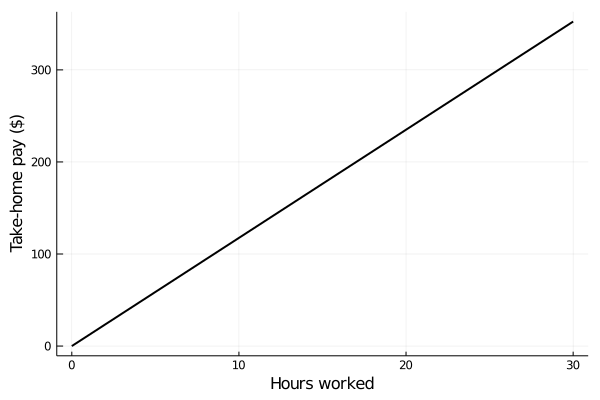
\includegraphics[width=0.45\textwidth]{linear.png}
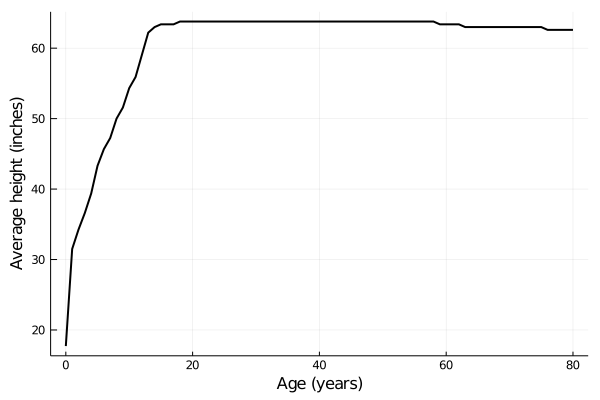
\includegraphics[width=0.45\textwidth]{nonlinear.png}
\caption{Linear and non-linear functions.}
\label{fig:linearNLPlots}
\end{figure}

By contrast, suppose I wanted to predict how tall a typical American human
female would be based on her age. While it's true that for most age ranges the
two variables increase together (just as more hours-worked implies more
take-home pay, so does more years-on-earth implies more inches-off-the-ground),
the plot is no longer a straight line (see the right side of
Figure~\ref{fig:linearNLPlots}).

It's worth lingering for a moment on what linear \textit{means} and how it
colors our assumptions about what to expect. Imagine this conversation:

\begin{dialogue}

\speak{You} Hey boss, I know I'm normally only scheduled to work for 12 hours a
week, and I get 120 bucks for that. But I need to start saving up for a plane
ticket to see my grandparents, so I'd like to inch that up to 15 hours next
week. That okay?

\speak{Boss} Sure, you can do 15 next week. That'll make your take-home
pay an even \$5,000 for the week.

\speak{You} \direct{Jaw drops open} Whoa, five \textit{grand}?! Heck, in that
case, push me up to 20 -- I can make some headway on my fall tuition!

\speak{Boss} Twenty hours it is -- you'll earn a total of 75\textcent~for
that.

\speak{You} \textit{D'oh!!}

\end{dialogue}

The above dialogue is absurd. But exactly \textit{why} is it absurd? Answer:
because we expect weekly-pay-vs.-hours-worked to be linear, and the values
given in the dialogue violate our linear assumptions.

\bigskip
The following scene, by contrast, \textit{isn't} absurd:

\begin{dialogue}

\speak{You} It's now been 12 months since I bought it, and my Blackberry stock
is currently worth \$120. Dear Crystal Ball, how much will it be worth three
months from now (the 15-month point)?

\speak{Crystal Ball} Blackberry will skyrocket in the public's imagination
three months from now, so at the 15-month mark your stock will be valued at
\$5,000.

\speak{You} Woo-hoo! And how about at the 20-month mark?

\speak{Crystal Ball} Unfortunately for shareholders, Blackberry Inc.~will make
some bad business decisions and crash. The stock will be nearly worthless --
just 75\textcent.

\speak{You} Yikes -- glad I asked! Please sell it in three months, okay?

\end{dialogue}

This scenario doesn't seem out of the question because we have no expectations
about stock prices being linear in time.

\medskip

So what exactly are those linear expectations? If you work it out, they come
down to two:

\definecolor{shadecolor}{rgb}{.9,.9,.9}
\begin{framed}
If a function $f(x)$ is linear, then:
\begin{compactitem}
\item $f(a\cdot x)$ is always simply $a\cdot f(x)$.
\item $f(x+y)$ is always simply $f(x)+f(y)$.
\end{compactitem}
\end{framed}

Take the first one. Let's say Wawa is selling a King Size Kit Kat bar for
\$1.50. How much would four bars cost? The answer's got to be \$6.00. It would
be weird to be anything else. In this example, if $x$ is the number of Kit Kat
bars, and $f(x)$ is the total cost. $f(x) = 1.5x$, and predictably, $f(4\cdot
1) = 4 \cdot f(1) = 4 \cdot 1.5 = 6.$

For the second rule, let's say we bought two Kit Kat bars today and three more
tomorrow. How much for the total? If the universe is working normally, buying
two today and three tomorrow would be the same price as buying five altogether.
And it's true: $f(2+3) = f(2) + f(3) = 3 + 4.5 = 7.5 = f(5)$. It would be weird
to work any other way.

When we have non-linear functions, we don't expect these things to be true. If
my nine-year old daughter is 4 feet tall, I don't expect her to be 8 feet tall
when she turns eighteen. $f(a\cdot x) \neq a\cdot f(x)$. And if my Blackberry
stock is worth \$5,000 after sixteen months and \$100 after the company's
disastrous seventeenth, we don't count on it being worth \$5,100 after 33
months. $f(x+y) \neq f(x)+f(y)$.

For the rest of this entire book, the two assumptions above will always be
true. It may seem limiting, but as we've seen, there are lots of cases where it
simply doesn't make any sense for our function \textit{not} to be linear.

\section{This book contains only elephants}

\index{elephants}
\index{Ulam, Stanis\l{}aw}

The great mathematician and computational scientist Stanis\l{}aw Ulam once
quipped that dividing functions into linear and non-linear is like dividing
zoology into ``elephant'' and ``non-elephant.'' In a way it's true, because
there are certainly far more functions that \textit{don't} obey the above two
properties than there are those that do. By the same token, though, there are
far more pay schemes we could invent than just ``a regular hourly rate.'' But
hourly rates come up very, very often, and when they do, there's a lot of
amazingly useful things we can do with them. Join us on our hike and you'll
see.



% TODO: appendix with Python

% TODO: somewhere in this chapter, I should do the parachute illustration with
% the gravitational force and the cross-wind force and the momentum from the
% airplane force. But where?

% TODO: introduce the notation R^3 for a 3-dimensional vector of reals. (Note:
% I do talk about this in linearTrans chapter, so forward/backward reference
% from there.)

\chapter{Vectors}

\index{vector}
As I stated on p.~\pageref{mathematicalObject}, every ``algebra'' is comprised
of a set of mathematical objects which you can combine with various operations.
In linear algebra, those building blocks are \textbf{vector}s and
\textbf{matrices} (singular: matrix). Buried within them are many mysteries.
We'll cover them in considerable detail in this chapter and the next.

\section{Vector vs.~scalar quantities}

\index{scalar}
\index{scale of measure}

The first thing we should do is perhaps distinguish between a vector quantity
and a \textbf{scalar quantity}, which probably had the spotlight in most of
your previous math classes. A scalar value is simply a \textit{single} number,
like 5, or -3.2, or $\pi$, or even $9 + 2i$ if you're into imaginary numbers.
The word \textit{scalar} is related to the word \textit{scale}, as in a ``scale
of measure.'' Think of stepping on a scale to weigh yourself in the morning:
your scale gives you back a single number (which you may or may not like; I
won't judge).

\index{one-dimensional quantity}
\index{dimension}

We'll call scalars \textbf{one-dimensional} values. That might seem odd, since
we haven't really talked about ``dimensions,'' yet. But think of the plain-old
\textbf{number line} you learned about back in elementary school. Zero's drawn
in the middle, positive numbers to the right and negative numbers to the left,
and the whole thing extends infinitely in just one direction\footnote{It might
seem like ``two directions,'' since the number line goes both to the left and
to the right. But since \index{left-ness} \index{right-ness} left-ness is the
exact opposite of right-ness, these are considered ``the same direction''; it's
just a matter of how far you go back or forth you go along that one straight
path.}.

% TODO: draw number line

\index{tuna fish}
\index{stock price}

Examples are so ubiquitous they're hardly worth mentioning. A person's weight
in the morning is a scalar. A company's stock price on a given day is a scalar.
So is the net \textit{movement} (up or down) of a stock's price from one day to
the next. So is a respondent's answer to the survey question ``on a 1-to-10
scale, how much do you enjoy tuna fish?'' You can think of countless others.

We of course often use variables to represent scalar quantities, and in this
book we'll put a variable in italics (like ``\textit{x}'' or
``\textit{price}'') to signify that its underlying value is a scalar quantity.

\subsection{A vector: a multi-dimensional quantity}
\index{vector}

Now a vector quantity is kind of the same thing, except that it represents
\textit{more than one} value. Suppose we wanted to represent not just a stock's
price on a given day, but an entire year's worth of prices on consecutive days.
Then, we would need a vector quantity. Instead of a survey respondent's answer
to just one question, we might want to store her entire set of answers to all
twenty questions on the survey. Instead of tracking just my weight, I might
want to record my weight, height, BMI (body-mass index), and pulse, all at a
given moment.

\index{losing information}
\index{information loss}

Vectors are \textbf{multi-dimensional} quantities. And they can't be
represented on a number line. Let's say my weight is 210 lbs.~and my height is
6'2", or 74 inches. (This is not theoretical.) I could of course draw a number
line and put a dot at 74 and another dot at 210, but this wouldn't fully
represent the fact that my weight was 210 and my height was 74. For one thing,
the numbers are on completely different scales. (There's that word ``scale''
again.) For another, it's not clear which is which -- is the right-most point
supposed to be my height, or my weight? Trying to squeeze a two-dimensional
quantity into a one-dimensional number line would \textbf{lose information.}
We need a representation scheme that can accommodate the complexity of our
quantity.

\index{Cartesian plane}
\index{coordinate plane}

For a two-dimensional quantity like weight-and-height, the obvious choice is
the two-dimensional Cartesian plane. I've drawn the vector with my height and
weight on the left side of Figure~\ref{fig:vector}. You'll see that there's an
\textit{arrow} from the origin to the point (210,74), rather than just a
circular dot at that point, as you might have expected. This is because
sometimes, it turns out, we want to treat a vector as ``a net movement in a
particular direction for a particular distance.''


\begin{figure}[ht]
\centering
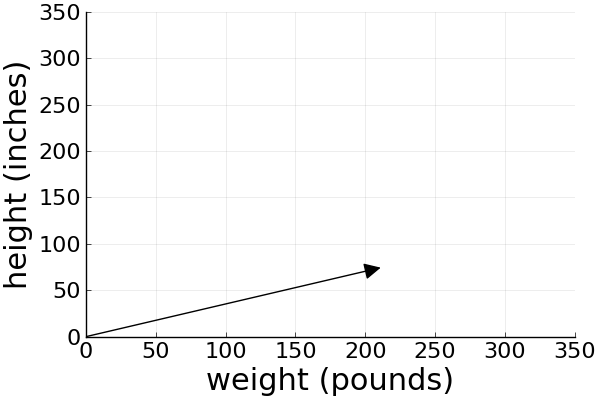
\includegraphics[width=0.4\textwidth]{vector.png}
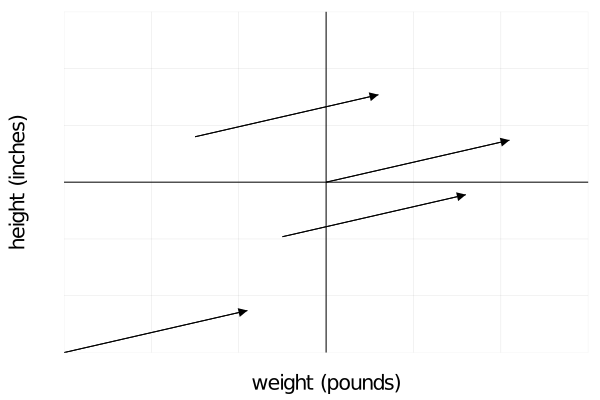
\includegraphics[width=0.58\textwidth]{vectors.png}
\caption{Left: a two-dimensional vector, depicted in a Cartesian plane. Right:
several copies of \textit{the same vector}, shown originating at various
points. They're considered ``the same'' vector because they all go in the same
direction and have the same length; the point they start at is irrelevant.}
\label{fig:vector}
\end{figure}

\index{magnitude (of a vector)}
\index{length (of a vector)}
\index{point of origin}
\index{direction (of a vector)}
\index{tail (of a vector)}
\index{tip (of a vector)}
\index{Stark, Arya}

You can see this illustrated on the right-hand side figure, where I've drawn
several copies of \textit{the same vector}. This may seem weird, but in terms
of pictures, here's how you want to think of it: \textbf{a vector has a
direction and a magnitude, but not a starting point}. The direction is the
specific angle in which it points, and (for now) we use the word
``\textbf{magnitude}'' to mean how long the vector is from its \textbf{tail} to
its \textbf{tip}. (As Arya Stark would say, the tip is the ``pointy end'' with
the arrowhead.) Curiously, there are alternative ways of judging the length, or
magnitude, of a vector, which we'll revisit in section~\ref{sec:norms}.

\index{counter-clockwise}

In the case of Stephen's biometric vector, its direction is
east-by-northeast-ish (about 19.4\textdegree\ counter-clockwise from the
$x$-axis) and its magnitude is 222.6. But it doesn't have any intrinsic ``point
of origin''; it's just an arrow pointing this-a-way and yea-far, no matter
where it might be anchored.

\index{mosquito}

Interestingly, the word \textit{vector} comes from a root meaning ``to carry.''
You may have heard people describe mosquitoes as being ``vectors'' for a
particular disease -- this means that they carry that disease. By thinking of a
vector as an arrow like in Figure~\ref{fig:vector}, the ``carry''
interpretation might start to make sense. A vector can represent a
transposition from one point to another. If I grew 74 inches taller and gained
210 more pounds, my point on the Cartesian plane would move in the direction
and the distance of that arrow.

\subsection{Don't visualize this}

Now that was all for \textit{two} dimensions. What about vectors with three, or
five, or even twenty dimensions? Well, for the three-dimensional case you can
indeed draw a 3-d figure with three axes, and plot three-dimensional points on
it. It turns out that most humans, though, are positively horrible at
interpreting such plots. And when you move beyond three dimensions, it's
utterly hopeless. (A friend of mine in fourth grade claimed he could visualize
four dimensions in his head, but I didn't believe him and still don't.)

But importantly, that doesn't mean we won't ever deal with higher-dimensional
vectors. In fact, vectors with lots and lots of dimensions will come up
constantly for us in this book -- believe it or not, we'll do an example where
the vectors have 50,000 dimensions! :-O

Don't worry; this won't make your head explode. In fact, it's a lot easier than
you might think to work with very high-dimensional vectors. Consider the
example I gave above about tracking a company's stock price every day for a
year. That's just a list of 365 numbers, all in a row. How hard is that to
imagine?

To work with vectors of more than three dimensions, you only have to do one
thing: give up trying to visualize them in a geometric space. As I'll describe
in the next section, it only occasionally makes sense to think about vectors
geometrically anyway; much of the time, we'll simply think of them as
quantities that have more than one component, unlike their simple brethren the
scalars.

\smallskip

Finally, the notation we'll use for vector variables. Instead of putting the
variable name in italics, we'll put it in bold-face with an arrow on the top of
it, like this: $\overrightarrow{\textbf{x}}$. The individual components of the
vector will be listed in boxies (square-brackets) like this: $[\ -2\ \ 5.9\ \
17\ \ -3\ ]$. So, if we define $\overrightarrow{\textbf{stephen}}$ as the
vector with my height and weight in it, we would write:

\vspace{-.15in}

\begin{align*}
\overrightarrow{\textbf{stephen}} = [\ 210\ \ 74 \ ].
\end{align*}

\medskip

\section{Five ways to think about vectors}

\begin{figure}[ht]
\centering
\includegraphics[width=1\textwidth]{fiveWays.pdf}
\caption{Five ways to think about a vector.}
\label{fig:fiveWays}
\end{figure}


In the mathematical writings you'll encounter, computer scientists use the word
``vector'' in a variety of ways. They're all ultimately compatible with each
other, but they can seem disorientingly different at first. Really, it's a
tribute to how powerful the vector concept is that people use them in so many
ways for so many different things.

I'm going to suggest that there are \textit{five} different ways to think about
a vector, and I'm going to arrange these ways on a continuum from ``concrete''
to ``abstract.'' This spectrum is depicted in Figure~\ref{fig:fiveWays}.

Let's take it from the bottom.

\subsection{1. A sequence of two coordinates}

\index{coordinate}
\index{element}
This is the height-weight example, in which something like
$\overrightarrow{\textbf{stephen}}$ is an ordered pair that can easily be
visualized on a two-dimensional Cartesian plane. Because of this plotting
aspect, I'll often call the two parts of the vector \textbf{coordinates}, but
as we create vectors with more pieces I'll more often call them
\textbf{elements}. These terms mean the same thing -- they both refer to the
individual components of the vector.

\index{index number}

We will need a way to select one of the coordinates individually, and for that
we use an \textbf{index number} (sometimes abbreviated to simply
``\textbf{index},'' the plural of which is ``indices.'') As you can see in
Figure~\ref{fig:fiveWays}, I've put two smaller numbers directly below the two
coordinates of the bottom vector, to indicate that we call them ``coordinate
\#0'' and ``coordinate \#1.'' We'll also use the phrase ``\textbf{index into
the vector},'' where ``index'' is a verb. If we take that bottom-most vector,
and index into it at coordinate 1, we get the (scalar) value 93.

Notation-wise, if we have a two-dimensional vector called
$\overrightarrow{\textbf{bob}}$, we'll often write $bob_0$ for the value of the
first coordinate and $bob_1$ for the second.

As an aside, you might wonder why the coordinates are numbered 0 and 1 instead
of 1 and 2. The answer has to do with the fact that we'll be using Python in
this book. Every programming language has a way of indexing into its
vector-like objects, and Python, Java, and C++ all begin indexing with the
number 0. There are actually some good reasons for this, which I won't get
into. It's not universally embraced, however; languages like R and Julia start
their indexing at 1. Go figure.

\index{tail (of a vector)}
\index{tip (of a vector)}
\index{radius@``radius''}
\index{Pythagorean Theorem}
\index{crow-flies distance@``crow-flies'' distance}

Geometrically, we can compute a vector's direction and magnitude using
trigonometry. Figure~\ref{fig:directionMag} shows a vector
$\overrightarrow{\textbf{v}} = [\ 9 \ \ 21\ ]$ pictorially. Its $0^\text{th}$
coordinate (a.k.a. $v_0$) is 9, measured on the $x$-axis, and $v_1$ is 21.
Traditionally, a two-dimensional vector's magnitude is called $r$ (for
``radius,'' I believe, although don't think about that too hard) and its
direction is called $\theta$ (``theta''). The magnitude is just the crow-flies
distance from the vector's \textbf{tail} to its \textbf{tip} (computed using
the Pythagorean Theorem) and the direction is the arctangent of the
rise-over-run. In equations:

\vspace{-.25in}
\begin{align*}
r &= \sqrt{v_0^2 + v_1^2} \\
\theta &= \tan^{-1} \frac{v_1}{v_0} \\
\end{align*}
\vspace{-.55in}

\begin{figure}[ht]
\centering
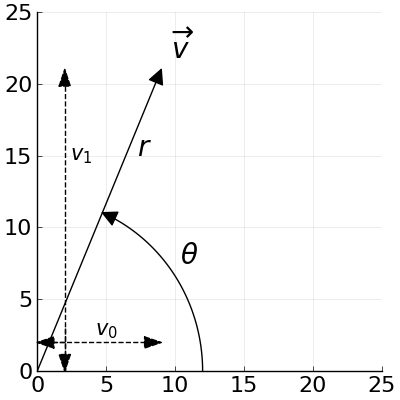
\includegraphics[width=.7\textwidth]{directionMag.png}
\caption[.]{The direction ($\theta$) and magnitude ($r$) of the vector
$\overrightarrow{\textbf{v}} = [\ 9 \ \ 21\ ]$. The direction $\theta$ is the
angle that $\overrightarrow{\textbf{v}}$ makes counter-clockwise with the
$x$-axis, and the magnitude is the length of the line.}
\label{fig:directionMag}
\end{figure}
\smallskip

\index{polar coordinates}
\index{Cartesian coordinates}

In this case, $r$ works out to 22.8 and $\theta$ is 66.8\textdegree. Think
about this, too: if, instead of giving you the values of $v_0$ and $v_1$, I
instead gave you the values of $r$ and $\theta$, you'd still have \textit{all
the information about the vector}, just in a different form. We sometimes call
$r$ and $\theta$ the \textbf{polar coordinates} of a vector, and $v_0$ and
$v_1$ the \textbf{Cartesian coordinates}. The polar coordinates are usually
written as ``$22.8 \measuredangle 66.8$\textdegree,'' which is the same vector
as $[\ 9 \ \ 21 \ ]$, just written in a different way.

Anyway, I put this way of thinking about vectors at the extreme ``concrete''
end of the spectrum, because it's so nuts-and-bolts and easy to visualize. As
we ascend up the hierarchy, things will get less and less visualizable.


\subsection{2. A sequence of more than two coordinates}

As I mentioned earlier in this chapter, having more than two coordinates in a
vector isn't really all that weird...you simply have to give up any hope of
visualizing it geometrically. But it's easy enough to do: a list of four
numbers -- 89, 93, 70, and 133 -- is the most natural thing in the world. One
could imagine finding the sum of the elements, the maximum element, the number
of negative elements, or other more exotic things.

Again, our indexing starts at 0, and this time goes up to 3. Note what this
implies: if we have a vector with four elements, there is no element \#4! This
is a common pitfall for newcomers to the subject and to languages like Python.
If I have a vector with $n$ coordinates, those coordinates are numbered 0 up to 
$n-1$, but \textit{not} up to $n$.

\index{dimension}
Also note that the number of elements/coordinates is also the
\textbf{dimensionality} (number of dimensions) of the vector. Simply put, a
vector that has nine elements in it is called ``a 9-dimensional vector.''

\subsection{3. A collection with non-numeric indices}

At this point of the hierarchy, I change my nomenclature from ``sequence'' to
``collection.'' That's because here, we don't \textit{number} the elements of
our vector anymore but instead \textit{name} them. Thus there isn't any
meaningful order to the elements anymore -- instead of ``IQ \#0,'' ``IQ \#1,''
and so forth, we have ``Jezebel's IQ,'' ``Filbert's IQ,'' and the like. Nothing
super weird here, but things may be starting to look less and less math-y to
you.

\index{label}

I'll sometimes call the names of the elements \textbf{label}s.

% TODO: talk about how diff languages represent this in diff ways; with R, you
% can name the elements of a vector, whereas in Python, you'll need a dict.

\subsection{4. A collection with non-numeric elements}

And heck, if the indices don't have to be numbers, why would the elements need
to be? And indeed we will often have cause to work with vectors like the one in
step 4 of the hierarchy (Figure~\ref{fig:fiveWays}, p.~\pageref{fig:fiveWays}),
in which there's not a number in sight. This example holds the favorite colors
for each of our four friends, which are of course non-numeric.

\subsection{5. Just a ``thing''}

Finally, you won't see this usage of vectors until you get to some more
advanced math, but I'd be doing you a disservice if I didn't point it out here.
I remember the first time I read some research in which the author was going on
and on about ``vectors,'' and I was dreadfully confused because none of his
``vectors'' seemed to have any elements in them! I was like, ``what do you mean
\textit{vectors}, dude? Did your word processor auto-correct a different
word?''

\index{vector space}
\index{algebra@``an algebra''}

This computer scientist was treating ``vectors'' as whole objects, not even
considering what their elements were (or whether they even \textit{had} any
elements). He was working with an abstract notion called a \label{vectorSpace}
\textbf{vector space} which we'll touch on next chapter; for now I'll just tell
you that it's closely related to the notion of an algebra that we discussed in
Chapter~\ref{ch:intro}. He was taking advantage of some of the elegant results
presented later in this book, which are guaranteed to hold for whatever
mathematical objects you care to define, as long as you obey certain ground
rules -- whether those objects have any ``elements'' to them or not. I mention
this mostly to anchor your future self in solid ground the first time you
inevitably come across the use of ``vector'' as a very un-list-like thing.
You'll remember reading this, say to yourself ``ah yes -- Stephen warned me
once that the extreme abstract end of the continuum works like this,'' and
proceed with confidence. I won't say anything more about it in this book.

\section{And a vector is also a function}

\index{function}
\label{vectorIsFunction}

Oh, and yet another way to think of vectors: as \textbf{function}s. We'll talk
about vectors as inputs to functions later in this book. But it's worth
recognizing at this point that a vector itself essentially \textit{is} a
function.

\index{domain}
\index{codomain}

You'll remember from Chapter 3 of \textit{Cool, Brisk Walk} that a function is
a mapping from a set of inputs to a set of outputs. Each member of the input
set (a.k.a. the ``domain'') is assigned a member of the output set
(``codomain'') as its value. (No member of the domain can be assigned to more
than one member of the codomain, but the reverse is not a constraint: multiple
members of the domain \textit{can} be assigned to the same member of the
codomain.)

Now consider this vector:

\begin{center}
\begin{tabular}{ccccccc}
$\overrightarrow{\textbf{x}} = [$ & 45 & -12 & 9 & 45 & 0 & $]$ \\
& \scriptsize{0} & \scriptsize{1} & \scriptsize{2} & \scriptsize{3} & \scriptsize{4}& \\
\normalsize
\end{tabular}
\end{center}
\vspace{-.15in}

It's a sequence of numbered elements, sure. But couldn't it just as easily be
interpreted as a function from index numbers to values? (See
Figure~\ref{vectorFunction1}.)

\begin{figure}[ht]
\centering
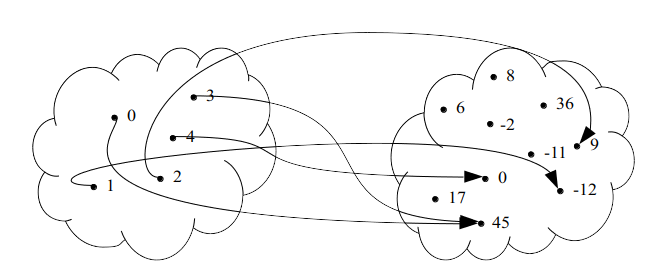
\includegraphics[width=1\textwidth]{vectorFunction1.png}
\caption[.]{The vector $\overrightarrow{\textbf{x}}$, interpreted as a function.}
\label{vectorFunction1}
\end{figure}

In function syntax, $\overrightarrow{\textbf{x}}(0) = 45$,
$\overrightarrow{\textbf{x}}(1) = -12$, $\overrightarrow{\textbf{x}}(3) = 45$,
and so on. It makes even more sense with a non-numeric vector like the
``favorite color'' example (Fig.~\ref{fig:fiveWays}), where
$\overrightarrow{\textbf{faveColor}}(\textrm{Biff}) = \textrm{blue}$ and
$\overrightarrow{\textbf{faveColor}}(\textrm{Betty Lou}) = \textrm{purple}$.
Instead of index numbers, the function's domain is comprised of the vector's
labels.

\index{ah-ha@``ah-ha"!''~moment}
\index{dictionary}
\index{hash table}
\index{array}
\index{associative array}
\index{list}
\index{vector}
\index{function}

I remember having a real ``ah-ha!''~moment the day I first realized that
vectors (called ``arrays'' or ``lists'' in some programming languages) were
really the same as key/value-pair-based associative arrays (also called
``dictionaries'' or ``hash tables'') with \textit{an index number as the key}.
Later, I had another ``ah-ha!''~and realized that both were equivalent to
functions as well, if you viewed the keys/indices as the function's domain and
the elements as the codomain. Wow. Sometimes it seems like the universe is
really all just one thing.

%Vectors in the wild
%
%
%time series
%
%temperatures over time
%
%
%
%items with attributes
%
%loan attributes: age, credit score, loan amount, salary
%
%
%
%MP3 file
%
%everything has to be in binary to be in a computer
%
%air displacement vs. time
%
%sampling
%
%
%
%image files
%
%BW vs color
%
%can do finding faces, brighten the image, whatever
%
%
%
%binary string of text
%
%plain-text, encrypt with key, to get cipher text
%
%
%
%
%Google, vector representation of web pages
%
%bag of words
%
%
%
%Emails, spam detectors
%
%
%
%matchmaker.com 
%
%
%
%Facebook:
%represent each vertex as a vector of people-he's-friends-with 
%
%
%Purchasing patterns, 
%recommender systems (collaborative filbert)
%
%
%
%system state, population growth


\section{Vector operations}
\label{vectorOps}

We're going to be combining scalars/vectors to yield other scalars/vectors like
literally all the time. The following three operations must be mastered until
you can do them in your sleep.

\subsection{Operation \#1: Scalar-vector multiplication}

\label{scalarVectorMultiplication}

What do you think you'd get if you multiplied a scalar like 2 by a vector like
$[\ 3\ \ 0\ \ 4\ ]$? As with all mathematics, we can define this operation to
be anything we want. A reasonable guess would be to take the scalar number of
copies of the vector, like so:

\vspace{-.15in}
\begin{align*}
2 \cdot [\ 3\ \ 0\ \ 4\ ] = [\ 3\ \ 0\ \ 4\ \ 3\ \ 0\ \ 4\ ] ? \quad  \quad
\textrm{NOPE}
\end{align*}
\vspace{-.15in}

But we're not doing to define it that way. Instead, we'll multiply the scalar
by each of the vector's elements individually, to get another vector with the
same number of elements:

\vspace{-.15in}
\begin{align*}
2 \cdot [\ 3\ \ 0\ \ 4\ ] = [\ 6\ \ 0\ \ 8\ ]
\end{align*}
\vspace{-.15in}

\index{scalar-vector multiplication}

This turns out to be more useful. So in general, a scalar $a$ times a vector
$\overrightarrow{\textbf{v}}$ will be:

\vspace{-.15in}
\begin{center}
\begin{framed}
\textbf{Scalar-vector multiplication:}
\begin{align*}
a \overrightarrow{\textbf{v}} = a [\ v_0\ \ v_1\ \ \dots \ \ v_{n-1}\ ] =
[\ a \cdot v_0\ \ a \cdot v_1\ \ \dots \ \ a \cdot v_{n-1}\ ],
\end{align*}
where $n$ is the number of elements in the vector.
\end{framed}
\end{center}
\vspace{-.15in}

Interestingly, there's no such thing (in common use) as ``scalar-vector
\textit{addition}.'' In other words, if someone tried to do this:

\vspace{-.15in}
\begin{align*}
2 + [\ 3\ \ 0\ \ 4\ ] = \ ??
\end{align*}
\vspace{-.15in}

\index{no can do@``no can do''}
we're simply going to say ``no can do.''

By the way, some programming languages (including Python) do give the
programmer a convenient shorthand by allowing them to type
$2 + [\ 3\ \ 0\ \ 4\ ]$ and get the value $[\ 5\ \ 2\ \ 6\ ]$. This isn't
considered a bona fide mathematical operation, though; just a notational
convenience.

\subsection{Operation \#2: Vector addition}

Adding two vectors together, though, is a perfectly acceptable enterprise,
provided that the vectors have the same number of elements. The way we do it is
to add each pair of elements together and produce another vector of the same
number of dimensions. In other words, adding $[\ 2\ \ 9\ ]$ to $[\ 4\ \ -2\ ]$
gives us:

\vspace{-.15in}
\begin{align*}
[\ 2\ \ 9\ ] + [\ 4\ \ -2\ ] = [\ 6\ \ 7\ ],
\end{align*}
\vspace{-.15in}

and in general:

\vspace{-.15in}
\begin{center}
\begin{framed}
\textbf{Vector addition:}
\begin{align*}
\overrightarrow{\textbf{x}} + \overrightarrow{\textbf{y}} &=
[\ x_0\ \ x_1\ \ \dots \ \ x_{n-1}\ ] +
[\ y_0\ \ y_1\ \ \dots \ \ y_{n-1}\ ] \\
&= [\ x_0 + y_0\ \ x_1 + y_1\ \ \dots \ \ x_{n-1} + y_{n-1}\ ],
\end{align*}
where $n$ is the number of elements in each vector.
\end{framed}
\end{center}
\vspace{-.15in}

An important issue arises in level 3 of our Figure~\ref{fig:fiveWays} hierarchy
(p.~\pageref{fig:fiveWays}). How do we add two vectors that aren't indexed by
number? Answer: we add the elements from each vector that correspond to the
same \textit{label}. And yes, the vectors must \textit{have} exactly the same
labels in order to be legitimately added in this way; otherwise, we call the
whole thing off. So:

\index{Mrs.~Peacock}
\index{Mr.~Green}
\index{Prof.~Plum}

\begin{center}
\begin{tabular}{ccccccccc}
[ & 3 & 5 & 8 & ] \ + \ [ & 1 & -6 & 4 & ] \ = \\
& \scriptsize{peacock} & \scriptsize{green} & \scriptsize{plum} & &
\scriptsize{peacock} & \scriptsize{green} & \scriptsize{plum} & \\
\normalsize
\end{tabular}
\vspace{-.15in}
\begin{tabular}{ccccc}
[ & 4 & -1 & 12 & ], \\
& \scriptsize{peacock} & \scriptsize{green} & \scriptsize{plum} & \\
\normalsize
\end{tabular}
\end{center}
\vspace{-.15in}

and

\index{Miss Scarlet}
\index{Mrs.~White}
\index{Col.~Mustard}

\begin{center}
\begin{tabular}{ccccccccc}
[ & 2 & 1 & 4 & ] \ + \ [ & 3 & 3 & 0 & ] \ = \\
& \scriptsize{scarlet} & \scriptsize{mustard} & \scriptsize{green} & &
\scriptsize{scarlet} & \scriptsize{white} & \scriptsize{plum} & \\
\normalsize
\end{tabular}

\index{no can do@``no can do''}
\vspace{-.15in}
``no can do.''
\end{center}
\vspace{-.15in}

\index{commutative}
\index{distributive}

\medskip
You can probably tell that vector addition is \textbf{commutative}, meaning
that whether we add $\overrightarrow{\textbf{x}}$ +
$\overrightarrow{\textbf{y}}$ or $\overrightarrow{\textbf{y}}$ +
$\overrightarrow{\textbf{x}}$, we get the same answer. It's also true that
vector addition, combined with scalar-vector multiplication, is
\textbf{distributive}. This means:

\vspace{-.15in}
\begin{align*}
a (\overrightarrow{\textbf{x}} + \overrightarrow{\textbf{y}}) &=
a \overrightarrow{\textbf{x}} + a \overrightarrow{\textbf{y}}
\end{align*}
\vspace{-.15in}
and

\vspace{-.15in}
\begin{align*}
(a + b) \overrightarrow{\textbf{x}} &=
a \overrightarrow{\textbf{x}} + b \overrightarrow{\textbf{x}}
\end{align*}
\vspace{-.15in}

for any scalars $a$ and $b$ and vectors $\overrightarrow{\textbf{x}}$ and
$\overrightarrow{\textbf{y}}$. This is a useful fact to know, which we'll
sometimes rely on.

\medskip

By the way, you might wonder whether vector subtraction is a thing, and it is:
in fact it turns out to just use scalar multiplication by $-1$. So:

\vspace{-.15in}
\begin{center}
$\overrightarrow{\textbf{x}} - \overrightarrow{\textbf{y}} =
\overrightarrow{\textbf{x}} + (-1 \overrightarrow{\textbf{y}}) =$ \\
$ [\ x_0 - y_0\ \ x_1 - y_1\ \ \dots \ \ x_{n-1} - y_{n-1}\ ]$.
\end{center}

For example, $[\ 5\ \ 2\ \ 7\ ] - [\ 1\ \ 4\ \ 7\ ]$ is just $[\ 4\ \ -2\ \ 0\ ]$.

\subsection{Operation \#3: Vector multiplication (dot product)}

\label{dotProduct}
\index{dot product}
\index{cross product}

Our third and final vector operation is the least intuitive of the three; at
least, it doesn't work the way I expected it to when I first learned it. It's
most commonly called the \textbf{dot product}.\footnote{There is at least one
other type of vector multiplication in common use, which we won't need in this
book. It's called the \textbf{cross product}, and is designated by a $\times$
instead of a $\cdot$. Interestingly, although the dot product is defined for
vectors of any number of dimensions, the cross product is only defined for
vectors of exactly three dimensions. (Not 2. Not 4. Only exactly 3.) Another
curious fact is that the cross product between two vectors gives you a vector
back, not a scalar like the dot product does.}

The first thing you have to wrap your head around is the fact that \textit{two
vectors multiplied together give you a scalar.} Yeah, no cap: if you multiply
an 18-dimensional vector by another 18-dimensional vector, you get back a
single lonely number.

Operationally, what happens is that you \textit{multiply} the corresponding
elements of the two vectors together, and then \textit{add} the result. So:

\vspace{-.15in}
\begin{align*}
[\ 7\ \ 8\ ] \cdot [\ 5\ \ 1\ ] = 7\cdot 5 + 8\cdot1 = 43
\end{align*}
\vspace{-.15in}

As with vector addition, we disallow taking the dot product of two vectors with
differing numbers of elements. Also, in the case of vectors with labels instead
of index numbers, we insist that the vectors have identical labels in order to
meaningfully dot-product them.

\index{dot product}
\begin{center}
\begin{framed}
\textbf{Vector multiplication (dot product):}
\begin{align*}
\overrightarrow{\textbf{x}} \cdot \overrightarrow{\textbf{y}} &=
[\ x_0\ \ x_1\ \ \dots \ \ x_{n-1}\ ] \cdot
[\ y_0\ \ y_1\ \ \dots \ \ y_{n-1}\ ] \\
&= x_0 \cdot y_0\ + x_1 \cdot y_1\ + \dots + x_{n-1} \cdot y_{n-1},
\end{align*}
where $n$ is the number of elements in each vector.
\end{framed}
\end{center}
\vspace{-.15in}

\index{commutative}

It should be obvious to you that the dot product operation is commutative:
$\overrightarrow{\textbf{x}} \cdot \overrightarrow{\textbf{y}}$ always gives
the same result as $\overrightarrow{\textbf{y}} \cdot
\overrightarrow{\textbf{x}}$.

\subsubsection{Why?}

Okay, now to address the elephant in the living room: \textit{why} would
mathematicians define vector multiplication in this way? What's the matter with
just multiplying corresponding elements and yielding a vector answer, like we
did with vector addition?

The answer is that the dot product as defined above is incredibly useful, much
more so than pairwise-multiplication will turn out to be. In fact, it's
possibly the single most important calculation in linear algebra: all kinds of
applications and more advanced computations use it as a building block.

To see this, consider the following question. What needs to be true about two
vectors in order for them to have a large dot product?

Your first inclination might be to answer ``the individual vector entries need
to be large.'' This is sort of true...but only sort of. Consider the following
two vectors:

\vspace{-.15in}
\begin{align*}
\overrightarrow{\textbf{a}} &= [\ 95\ \ 0\ 381\  ] \\
\overrightarrow{\textbf{b}} &= [\ 0\ \ 1056\ 0\  ] \\
\end{align*}
\vspace{-.15in}

Thar's som' mighty big entries in them vectors. Surely multiplying them
together would give a large result, right? No:

\vspace{-.15in}
\begin{align*}
[\ 95\ \ 0\ 381\ ] \cdot [\ 0\ \ 1056\ 0\ ] &= \\
95 \cdot 0 + 0 \cdot 1056 + 381 \cdot 0 &= 0.
\end{align*}
\vspace{-.15in}

We get zilch. By contrast, these two wimpy-looking vectors:

\vspace{-.15in}
\begin{align*}
\overrightarrow{\textbf{c}} &= [\ 1\ \ 2\ \ 5\ ] \\
\overrightarrow{\textbf{d}} &= [\ 0\ \ 2\ \ 7\ ] \\
\end{align*}
\vspace{-.15in}

do give a fairly hefty result:

\vspace{-.15in}
\begin{align*}
[\ 1\ \ 2\ \ 5\ ] \cdot [\ 0\ \ 2\ \ 7\ ] &= \\
1 \cdot 0 + 2 \cdot 2 + 5 \cdot 7 &= 39.
\end{align*}
\vspace{-.15in}

What's going on here?

\medskip

If you stare at the above calculations, you'll hit on a deep truth which is
worth pondering at length. And that is that in order for the dot product to be
large, the vectors must not only have large entries, but be large \textit{in
the same places.}

The reason that $\overrightarrow{\textbf{a}}$ and $\overrightarrow{\textbf{b}}$
had such a stunningly low dot product is that although they had large entries,
they were completely out of sync with each other. $\overrightarrow{\textbf{a}}$
had high values precisely where $\overrightarrow{\textbf{b}}$ had low ones, and
vice versa. On the other hand, even though the individual elements of
$\overrightarrow{\textbf{c}}$ and  $\overrightarrow{\textbf{d}}$ were pretty
small, they fit together nicely: for example, $\overrightarrow{\textbf{c}}$'s
largest entry and $\overrightarrow{\textbf{d}}$'s largest entry were in the
same place (element \#2), which led to a kind of synergy.

Consider how the dot product would change if we altered
$\overrightarrow{\textbf{d}}$ to be $[\ 7\ \ 2\ \ 0\ ]$ instead of $[\ 0\ \ 2\
\ 7\ ]$:

\vspace{-.15in}
\begin{align*}
[\ 1\ \ 2\ \ 5\ ] \cdot [\ 7\ \ 2\ \ 0\ ] &= \\
1 \cdot 7 + 2 \cdot 2 + 5 \cdot 0 &= 11.
\end{align*}
\vspace{-.15in}

Dang, we dropped from 39 all the way to 11 just by reordering the entries. 

\index{Jezebel}
\index{matchmaker@\texttt{matchmaker.com}}
\label{matchmakerExample}

This ability to judge roughly ``how aligned'' two vectors are comes up all the
time. Consider a dating website. Let's say that Jezebel, a heterosexual female,
signs up for a dating service and answers the questions on a compatibility
survey. She's asked, ``on a scale of 1 to 10, how much do you like action
movies? Outdoor hikes? Candlelight dinners? Reading mystery novels?'' Suppose
her answers are the following:

\begin{center}
\begin{tabular}{cccccc}
$\overrightarrow{\textbf{jezebel}}$ = [ & 5 & 2 & 10 & 2 & ] \\
& \scriptsize{action} & \scriptsize{hiking} & \scriptsize{candlelight} &
\scriptsize{mystery} & \\
\normalsize
\end{tabular}
\end{center}
\vspace{-.15in}

\index{Filbert}
\index{Wendell}
\index{Biff}

Now there are three eligible heterosexual bachelors on this site: Biff,
Filbert, and Wendell. They also took the survey, and came up with these
responses:

\begin{center}
\begin{tabular}{cccccc}
$\overrightarrow{\textbf{biff}}$ \quad \ = [ & 10 & 10 & 1 & 1 & ] \\
& \scriptsize{action} & \scriptsize{hiking} & \scriptsize{candlelight} &
\scriptsize{mystery} & \medskip \\

$\overrightarrow{\textbf{filbert}}$ \ = [ & 6 & 2 & 8 & 4 & ] \\
& \scriptsize{action} & \scriptsize{hiking} & \scriptsize{candlelight} &
\scriptsize{mystery} & \medskip \\

$\overrightarrow{\textbf{wendell}}$ = [ & 1 & 3 & 3 & 10 & ] \\
& \scriptsize{action} & \scriptsize{hiking} & \scriptsize{candlelight} &
\scriptsize{mystery} & \\
\normalsize
\end{tabular}
\end{center}
\vspace{-.15in}

\index{matchmaker@\texttt{matchmaker.com}}
The central question that \texttt{matchmaker.com} must ask is: which of these
three young gentlemen should be recommended to Jezebel?

\smallskip

The answer lies in the dot product. Just by eyeballing the survey results, you
can probably tell that Filbert is Jezebel's best match: he has high values in
roughly the same place that she does. If we compute the dot product of Jezebel
with each of the three guys, we see that the math bears that out:

\begin{align*}
\overrightarrow{\textbf{jezebel}} \cdot \overrightarrow{\textbf{biff}} &=
5 \cdot 10 + 2 \cdot 10 + 10 \cdot 1 + 2 \cdot 1 = 82 \\
\\
\overrightarrow{\textbf{jezebel}} \cdot \overrightarrow{\textbf{filbert}} &=
5 \cdot 6 + 2 \cdot 2 + 10 \cdot 8 + 2 \cdot 4 = 122 \\
\\
\overrightarrow{\textbf{jezebel}} \cdot \overrightarrow{\textbf{wendell}} &=
5 \cdot 1 + 2 \cdot 3 + 10 \cdot 3 + 2 \cdot 10 = 61 \\
\end{align*}

Since Filbert has the highest dot product with Jezebel, Filbert's vector is in
some sense ``more closely aligned'' with hers, reflecting their similar
interests. So our website will show Filbert's pic and profile to Jezebel.

\medskip

\index{Mr.~Right}

It might occur to you that someone could ``beat the system'' here by answering
10 on all their survey questions. After all, increasing the individual entries
in a vector can't \textit{hurt} its dot product with another vector; the worst
it could do is not help matters, if the second vector has a zero there. So
let's say the insidious Mr.~Right (?) creates an account on the system, and
answers:

\begin{center}
\begin{tabular}{cccccc}
$\overrightarrow{\textbf{mrright}}$ \quad \ = [ & 10 & 10 & 10 & 10 & ] \\
& \scriptsize{action} & \scriptsize{hiking} & \scriptsize{candlelight} &
\scriptsize{mystery} & \medskip \\
\normalsize
\end{tabular}
\end{center}
\vspace{-.15in}

Pairing him with Jezebel yields:

\vspace{-.15in}
\begin{align*}
\overrightarrow{\textbf{jezebel}} \cdot \overrightarrow{\textbf{mrright}} &=
5 \cdot 10 + 2 \cdot 10 + 10 \cdot 10 + 2 \cdot 10 = 190 \\
\end{align*}
\vspace{-.25in}

which blows away the competition. Mr.~Right can have any girl he wants, whether
or not he and she are truly compatible. There's a way to fix this, which we'll
see later in this chapter (section~\ref{normalizing},
p.~\pageref{normalizing}). For now, just grasp the main point that two vectors
having large entries in the same places tends to magnify their dot product.

\bigskip
\bigskip
\phantom{.}

\subsection{Geometric interpretation}

Now let's build some \textit{geometric} intuition about the dot product.
Consider the two vectors $\overrightarrow{\textbf{a}}$ and
$\overrightarrow{\textbf{b}}$ in Figure~\ref{fig:dotproduct1}.
$\overrightarrow{\textbf{a}}$ is the vector $[\ 2\ \ 0\ ]$ and
$\overrightarrow{\textbf{b}}$ is $[\ 0\ \ 3\ ]$. What is their dot product?
$2\cdot 0 + 0\cdot 3 = $ a big fat zero.

\begin{figure}[ht]
\centering
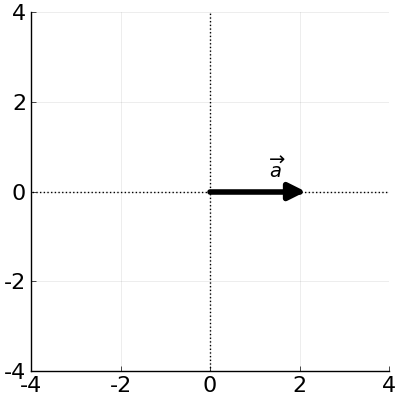
\includegraphics[width=0.45\textwidth]{dotProduct1a.png}
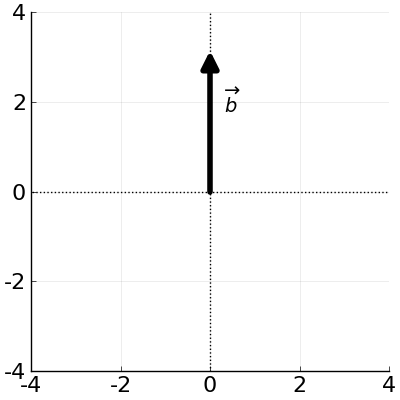
\includegraphics[width=0.45\textwidth]{dotProduct1b.png}
\caption{Two vectors whose dot product is 0.}
\label{fig:dotproduct1}
\end{figure}

\bigskip
Okay, same exercise, but now in Figure~\ref{fig:dotproduct2}. Now we have the
vectors $\overrightarrow{\textbf{a}} = [\ 3\ \ 3\ ]$ and
$\overrightarrow{\textbf{b}} = [\ -2\ \ 2\ ]$. What is their dot product? Once
more, zero: $3\cdot -2 + 3\cdot 2 = 0$.

\begin{figure}[ht]
\centering
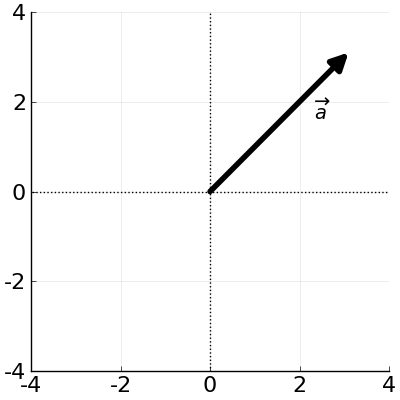
\includegraphics[width=0.45\textwidth]{dotProduct2a.png}
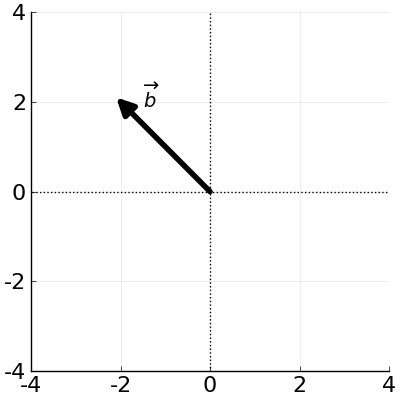
\includegraphics[width=0.45\textwidth]{dotProduct2b.png}
\caption{Another two vectors whose dot product is 0.}
\label{fig:dotproduct2}
\end{figure}

\bigskip
One more chorus. Figure~\ref{fig:dotproduct3} shows the
vectors $\overrightarrow{\textbf{a}} = [\ 1\ \ -2\ ]$ and
$\overrightarrow{\textbf{b}} = [\ -4\ \ -2\ ]$. What is their dot product? Yet
again, exactly zero: $1\cdot -4 + -2\cdot -2 = 0$.

\begin{figure}[ht]
\centering
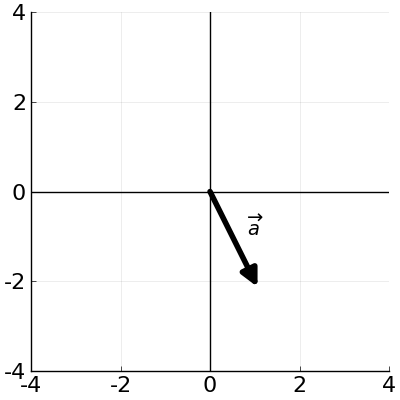
\includegraphics[width=0.40\textwidth]{dotProduct3a.png}
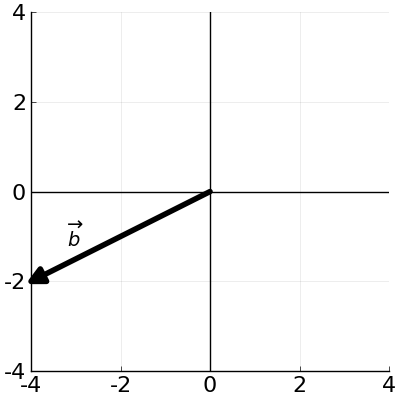
\includegraphics[width=0.40\textwidth]{dotProduct3b.png}
\caption{Yet another two vectors whose dot product is 0.}
\label{fig:dotproduct3}
\end{figure}

\bigskip

\index{perpendicular}
\index{orthogonal}
\index{right angle}

Three pairs of vectors, all of which have zero dot products. Now what's common
to all three examples? Answer: \textit{the vectors are perpendicular to each
other.} This is easier to see when we plot each pair on the same graph, as in
Figure~\ref{fig:allTogether}.

\begin{figure}[ht]
\centering
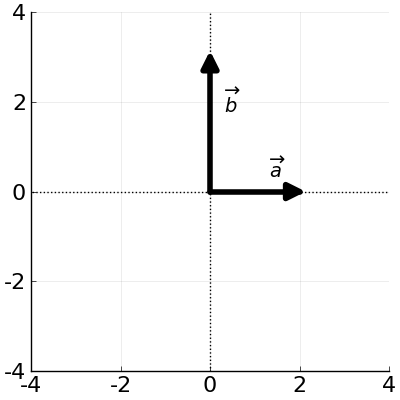
\includegraphics[width=0.31\textwidth]{dotProduct1.png}
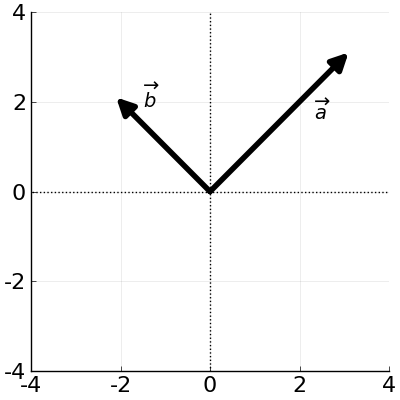
\includegraphics[width=0.31\textwidth]{dotProduct2.png}
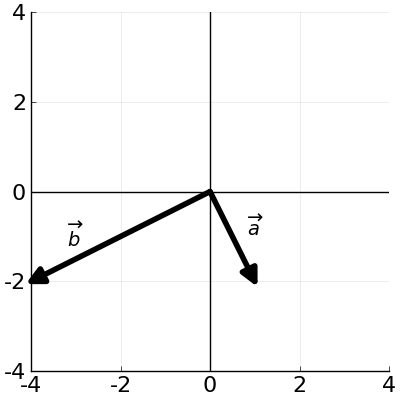
\includegraphics[width=0.31\textwidth]{dotProduct3.png}
\caption{The three pairs of vectors plotted together. The fact that they are
orthogonal to each other is what makes their dot products zero.}
\label{fig:allTogether}
\end{figure}

Whenever you have two vectors at exactly right angles to each other, their dot
product will be at a minimum; namely, zero. Our linear algebra term for this,
annoyingly, is not ``perpendicular'' (a word you already know) but
\textbf{orthogonal}. When two vectors are orthogonal, they're ``as unaligned as
possible.''

Think of it this way. Pick any of the three pairs of vectors in
Figure~\ref{fig:allTogether}, and pretend that your goal is to go in the
$\overrightarrow{\textbf{b}}$ direction. You want to get ``as b-ward as
possible.'' But suppose your only option was to go in the direction of
$\overrightarrow{\textbf{a}}$. Would you make any meaningful progress towards
your goal? The answer is no: $\overrightarrow{\textbf{a}}$ is exactly the
direction that doesn't let you move \textit{anywhere} you want to go. On the
left-most figure, for example, if your goal was to get from the origin due
north to the point $(0,15)$, you can't make any progress whatsoever if you're
allowed only to travel along the $x$-axis. And that's true for all three of
those pairs.

To get a non-zero dot product, the two vectors at least have to point
\textit{somewhat} in the same direction. Take the two in
Figure~\ref{fig:dotProduct4}, where $\overrightarrow{\textbf{a}} = [\ 3\ \ -3\
]$ and $\overrightarrow{\textbf{b}} = [\ 2\ \ -4\ ]$. These vectors are clearly
\textit{not} orthogonal, and hence their dot product is non-zero: $3\cdot 2 +
-3\cdot -4 = 18$.

\begin{figure}[ht]
\centering
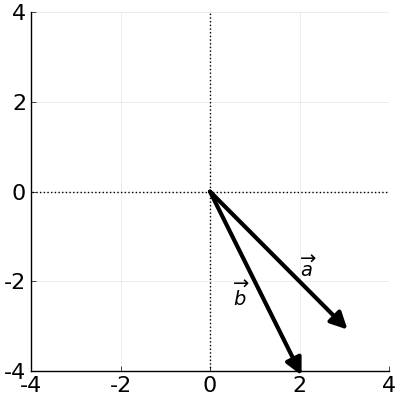
\includegraphics[width=0.80\textwidth]{dotProduct4.png}
\caption{Two \textit{non}-orthogonal vectors, whose dot product is 18.}
\label{fig:dotProduct4}
\end{figure}

In general, the more the arrows point in the same direction, the higher the dot
product, holding everything else equal. The more they diverge to right angles,
the more the dot product drops to zero. I'll have more to say about this in
Section~\ref{sec:norms} when we look at an alternate way to compute the dot
product geometrically.



\section{The vector operations in action}

This book is chock full of examples of using vectors in the real world. Let me
give one now which illustrates the eminent usefulness of these three vector
operations.

\smallskip
\label{bakeSale}
Let's say we've been tasked with baking goodies for a bake sale. There are
three recipes we're planning on making in bulk: chocolate chippers (my personal
fave), brownies, and fudge. Upon consulting our recipe book, we write down an
ingredient list for each:

\index{bake sale}
\index{brownies}
\index{fudge}
\index{chocolate chip cookies}

\begin{center}
\begin{tabular}{ccccccc}
$\overrightarrow{\textbf{chippers}}$ \ = [ & 2 & 1 & 1 & 1 & 3 &] \\
& \scriptsize{butter} & \scriptsize{sugar} & \scriptsize{chips} &
\scriptsize{flour} & \scriptsize{eggs} \smallskip \\
$\overrightarrow{\textbf{brownies}}$ \ = [ & 1 & 1 & 4 & 2 & 2 &] \\
& \scriptsize{butter} & \scriptsize{sugar} & \scriptsize{chips} &
\scriptsize{flour} & \scriptsize{eggs} \smallskip \\
\ \ $\overrightarrow{\textbf{fudge}}$ \quad \ = [ & 2 & 2 & 4 & 0 & 0 &]. \\
& \scriptsize{butter} & \scriptsize{sugar} & \scriptsize{chips} &
\scriptsize{flour} & \scriptsize{eggs} \bigskip \\
\end{tabular}
\end{center}
\vspace{-.05in}

This shows, for each of our five ingredients, how many ``units'' of each one is
required for one recipe's worth.\footnote{Warning: do \textit{not} attempt to
use these ingredient lists to actually make real goodies! I have left many
things out for simplicity. These would taste ratchet if you made them. Consult
a real recipe book.} Chocolate chip cookies evidently require two sticks of
butter, one cup of sugar, one package of Ghirardelli chocolate chips,
\textit{etc.}

\medskip

Additionally, we define these two vectors:
\index{fat, saturated}
\index{saturated fat}
\index{Wegmans}
\index{shopping list}

\begin{center}
\begin{tabular}{ccccccc}
$\overrightarrow{\textbf{wegmans}}$ \quad \ = [ & 1.59 & 2.79 & 3.49 & 1.67 &
.4 &] \\
& \scriptsize{butter} & \scriptsize{sugar} & \scriptsize{chips} &
\scriptsize{flour} & \scriptsize{eggs} \medskip \\
$\overrightarrow{\textbf{satfat}}$ \quad \ = [ & 56 & 0 & 24 & 1 & 1.6 &] \\
& \scriptsize{butter} & \scriptsize{sugar} & \scriptsize{chips} &
\scriptsize{flour} & \scriptsize{eggs} \medskip \\
\normalsize
\end{tabular}
\end{center}
\vspace{-.15in}

The first shows how much each of these ingredients is currently selling for at
Wegmans. For the health-conscious, the second shows how many grams of
saturated fat is present in each unit of the various ingredients. (*shudder*)

\medskip
Now, let's consider some common questions we might need to answer:

\begin{enumerate}
\itemsep1.5em
\item ``If we want to bake five batches of chocolate chippers for our bake sale,
what's on our shopping list?''

The answer is a simple vector operation:

% TODO: make this not look ratchet:

\vspace{.2in}
$\overrightarrow{\textbf{shoppinglist}}$ = 5 
$\overrightarrow{\textbf{chippers}}$
\vspace{-.15in}
\begin{center}
\begin{tabular}{rlcccccc}
&\quad\quad= [ & 10 & 5 & 5 & 5 & 15 &] \\
&& \scriptsize{butter} & \scriptsize{sugar} & \scriptsize{chips} &
\scriptsize{flour} & \scriptsize{eggs} & \smallskip \\
\end{tabular}
\end{center}

Scalar-vector multiplication gives us exactly what we want: multiply the number
of recipes by each ingredient's per-recipe quantity.

\item ``We've decided on six recipes of brownies and fudge, plus a dozen
batches of chocolate chippers. What's on our shopping list?''
\label{shoppingListQuestion}

Putting vector addition into the mix (see what I did there?) gives us our
elegant answer:

\begin{center}
$\overrightarrow{\textbf{shoppinglist}}$ 
= 6 $\overrightarrow{\textbf{brownies}}$
+ 6 $\overrightarrow{\textbf{fudge}}$
+ 12 $\overrightarrow{\textbf{chippers}}$

\begin{tabular}{rlcccccc}
&\quad\quad\quad\quad  = [ & 42 & 30 & 60 & 24 & 48 &] \\
&& \scriptsize{butter} & \scriptsize{sugar} & \scriptsize{chips} &
\scriptsize{flour} & \scriptsize{eggs} & \smallskip \\
\end{tabular}
\end{center}

\item ``My recipe tells me there are 16 brownies in a batch. How much saturated
fat is in each brownie?''

\index{dot product}

Here's where the dot product comes in handy. We have a vector
($\overrightarrow{\textbf{brownies}}$) that gives us the amount of each
ingredient, and another ($\overrightarrow{\textbf{satfat}}$) that gives us
per-unit fat content. The dot product is just what we need: multiply each
ingredient amount by its fat content, and add up the results. It's a snap! All
we then need to do is find the per-serving total by taking only a sixteenth of
a batch, which is scalar-vector multiplication again. Putting it all together:

\begin{align*}
\textit{fatPerBrownie} &=
\frac{1}{16} (\overrightarrow{\textbf{brownies}} \cdot
\overrightarrow{\textbf{satfat}}) \\[10pt]
&= \frac{1}{16} (1\cdot 56 + 1\cdot 0 + 4\cdot 24 + 2\cdot 1 + 2\cdot 1.6)
\smallskip \\[10pt]
&= 9.825\  \textrm{grams}.
\end{align*}

Ouch. Better sneak just one of those.

\item Finally, ``how much is this all going to cost me at Wegmans?''

We already computed the grand shopping list in
question~\ref{shoppingListQuestion}, above. To get the cost of this list, we
again simply use the dot product:

\begin{align*}
\textit{totalCost} &=
\overrightarrow{\textbf{shoppinglist}} \cdot
\overrightarrow{\textbf{wegmans}} \\[5pt]
&= 42\cdot 1.59 + 30\cdot 2.79 + 60\cdot 3.49 + 24\cdot 1.67 + 48\cdot .4
\smallskip \\[5pt]
&= \$419.16.
\end{align*}

Wowza: I sure hope we sell all these!

\end{enumerate}

Hopefully this gives you a feel for why the three operations -- and especially
the dot product -- are eminently useful. They turn out to be exactly what we
want to do with vectors much of the time, which is why they were invented. Get
to know them intimately.

\section{More about magnitude}
\label{sec:norms}

\index{tip (of a vector)}
\index{tail (of a vector)}
\index{Pythagorean Theorem}
\index{Euclidean distance}
\index{crow-flies distance@``crow-flies'' distance}

Flip for a moment back to Figure~\ref{fig:directionMag} on
p.~\pageref{fig:directionMag}. You'll recall that we defined the ``magnitude''
of the $\overrightarrow{\textbf{v}}$ vector as $r$: the crow-flies distance
from its tail to its tip, as computed by the Pythagorean Theorem. In that case,
we computed $r = \sqrt{v_0^2 + v_1^2} = 22.8$ for
$\overrightarrow{\textbf{v}}$'s magnitude.

Now like all of mathematics, we can define things however we want. It turns out
that this crow-flies distance thing -- also called the \textbf{Euclidean
distance} after Euclid, the ancient Greek geometer -- is only one possible way
to define the ``length'' or ``magnitude'' of a vector. This section includes
several others which prove useful in various settings.

\index{norm (of a vector)}
% TODO: put notation in index
\index{double-pipe sign@double-pipe sign ($\norm{\cdot}$)}

Oh, and before we get started, here's yet another piece of verbiage. The
preferred mathematical term for the sort of generalized magnitude measurement
presented below is the ``\textbf{norm}'' of a vector. We'll define several
different norms, each of which offers a different take on measuring a vector's
``size'' or ``bigness.'' No matter how we define it, \textit{the norm of a
vector is always a scalar}. We use double-pipe signs to represent it, like
this: $\norm{\overrightarrow{\textbf{v}}}$.

\subsection{The Euclidean (``$\boldsymbol\ell^\textbf{2}$'') norm}

The most common norm is the \textbf{Euclidean norm}, which is just what we
covered on p.~\pageref{fig:directionMag}. The Pythagorean Theorem is your
friend.

\index{cosine}
\index{dot product}

% TODO: talk more about cosine, even show a cosine curve

The Euclidean norm is used for many, many things, one of which is a second,
equally legitimate way to compute and to think about the dot product between
two vectors. First, recall the cosine operation from trigonometry. The cosine
of a 0\textdegree\ angle is 1, the cosine of a 90\textdegree\ angle is zero,
and in between those two extremes the cosine varies smoothly from 1 down to 0.

Now suppose we have a couple of two-dimensional vectors
$\overrightarrow{\textbf{a}}$ and $\overrightarrow{\textbf{b}}$. We'll use the
same ones from the example on p.~\pageref{fig:dotProduct4}, shown here in
Figure~\ref{fig:dotProduct4WithAngle}. To refresh your memory, the vector
$\overrightarrow{\textbf{a}}$ is $[\ 3\ \ -3\ ]$ and
$\overrightarrow{\textbf{b}}$ is $[\ 2\ \ -4\ ]$.


% TODO: add a second plot to this figure, showing two vectors with the same
% magnitudes as the existing plot, but with a bigger angle between them, and
% show how the dot product is less.
\begin{figure}[ht]
\centering
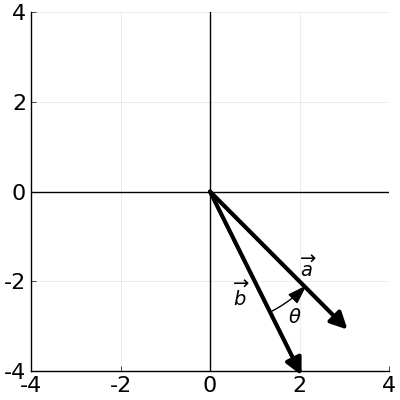
\includegraphics[width=0.6\textwidth]{dotProductWithAngle.png}
\caption{An alternate way to compute the dot product of two vectors, using the
angle between them in the calculation.}
\label{fig:dotProduct4WithAngle}
\end{figure}

We've learned that one way to compute the dot product between
$\overrightarrow{\textbf{a}}$ and $\overrightarrow{\textbf{b}}$ is to multiply
their corresponding entries:

\vspace{-.25in}
\begin{align*}
\overrightarrow{\textbf{a}} \cdot \overrightarrow{\textbf{b}} =
3\cdot2 + (-3)\cdot(-4) = 18.
\end{align*}
\vspace{-.25in}

Here's another way. We can \textit{multiply the two norms together, and then
multiply by the cosine of the angle between them.} You can really see why it's
called the dot ``product'' when you think of it this way. Multiplying vectors
is just multiplying their lengths...but there's a catch. We also multiply by
the cosine of their angle, so that the more they diverge from each other, the
lower the dot product.

In this example, we compute the angle between them (called $\theta$ in the
figure):

\vspace{-.2in}
\begin{align*}
\textrm{angle of } \overrightarrow{\textbf{a}} &= \tan^{-1} \frac{-3}{3} =
-45\degree\ \\
\textrm{angle of } \overrightarrow{\textbf{b}} &= \tan^{-1} \frac{-4}{2} =
-63.43\degree\ \\ 
\theta = \textrm{angle between } \overrightarrow{\textbf{a}} \textrm{ and }
\overrightarrow{\textbf{b}} &= -45\degree - (-63.43\degree) = 18.43\degree\ \\
\end{align*}

Now we can compute the dot product our new way:

\vspace{-.15in}
\begin{align*}
\overrightarrow{\textbf{a}} \cdot \overrightarrow{\textbf{b}} = 
\norm{\overrightarrow{\textbf{a}}} \cdot \norm{\overrightarrow{\textbf{b}}}
\cdot \cos
\theta &= \\
\sqrt{3^2+(-3)^2} \cdot \sqrt{2^2+(-4)^2} \cdot \cos 18.43\degree &= \\
4.243 \cdot 4.472 \cdot .948 & = 18. \\
\end{align*}

Yay! Same answer. I've found this a super useful way to visualize the dot
product, even though it's often more convenient to calculate it the original
way. A long vector times a long vector will give a large answer...provided
those long vectors are kinda sort pointing in the same direction. If they're
not -- and most especially, if they're at right angles to each other, a la the
Figure~\ref{fig:allTogether} examples (p.~\pageref{fig:allTogether}) -- then
the dot product can be miniscule even if the vectors themselves are long.

\bigskip

Okay, enough about the dot product. Back to the Euclidean norm itself. So far
we've been assuming two dimensions. But importantly, the Euclidean norm applies
equally well in \textit{any} number of dimensions. Suppose we had a
five-dimensional vector, like this one:

\begin{center}
$\overrightarrow{\textbf{f}} = [\ 3\ \ -4\ \ 5\ \ 17\ \ 0\ ]$.
\end{center}

The Pythagorean Theorem -- which in high school you may have only learned in a
two-dimensional setting -- still works just fine:

\begin{center}
$\norm{\overrightarrow{\textbf{f}}} =
\sqrt{3^2 + (-4)^2 + 5^2 + 17^2 + 0^2} = 18.412$.
\end{center}

Note: you still \textit{square} the entries and take the \textit{square} root
of the sum. (You don't take the fifth power of the entries and the fifth root
of the sum, like I expected when I first learned this.)

The result is (*deep breath*): ``the length of the straight line from the
origin to the point $(3,-4,5,17,0)$ in five-dimensional space.'' You can't
visualize it, so don't try. Just believe. No matter how many entries a vector
has, you can compute its crow-flies length this way.

Now for weird but ultimately consistent reasons, this Euclidean norm is also
called the ``$\ell^2$ norm''\footnote{Pronounced ``ell two,'' not ``ell
squared.''} of the vector. And we will sometimes write the 2 in as a subscript
to the double-pipe, like this:

\begin{center}
$\norm{\overrightarrow{\textbf{f}}}_2 = 18.412$.
\end{center}

I know it seems strange, but just go with it for now. And remember this, too:
if we \textit{don't} have any subscript after the $\norm{\cdot}$ signs,
\textit{the default is 2}. In other words, unless explicitly stated, the
``normal'' meaning of \textit{norm} is the $\ell^2$ norm, a.k.a. Euclidean
distance, computed by the Pythagorean Theorem.

\subsection{The Manhattan (``$\boldsymbol\ell^\textbf{1}$'') norm}

\index{Manhattan norm}
\index{taxicab norm}

% TODO: picture showing Manhattan distance and city blocks.

Imagine yourself in downtown Manhattan, New York City. You're a software
developer on an upper floor of the sleek new building at the corner of 33rd
Street and 8th Avenue. It's just about time for lunch, and you and your fellow
developers are discussing where to go -- the Thai place on 25th St.~and 10th
Ave.? The new Hungarian restaurant that opened up on 44th St.~and 6th Ave.? Or
will it be just the greasy subway shop four blocks uptown today?

One of the factors in your decision is the distance: you can't take forever for
lunch because you have a team meeting at 1:30pm. So you need to work out how
long it will take to walk (or take a taxicab) to each of these places. 

Now one (stupid) approach would be to use find the latitude and longitude of
both your office and each of the restaurants, and compute the Euclidean
distance. I say ``stupid'' because this is really only useful if you have a
helicopter. (We can dream.) In my world, you can't fly over buildings; you have
to walk around them. There's no point in computing the crow-flies distance if
you're not a crow.

So how do we determine the distance? Simple: it's just the number of blocks you
have to walk. Consider the Thai place. To get from 35th Street to 24th, we have
to walk five blocks. To get from 8th Avenue to 10th, we have to walk two.
Therefore, the walking distance between these two restaurants is ``ten
blocks.'' Note that it doesn't matter whether we walk the blocks west first and
then south, or south first and then west, or zig-zag back and forth between
streets and avenues: as long as we travel one of the shortest routes through
the buildings (which means never going east or north), it'll be ten blocks.

For reasons which should now be obvious, this way to measure distance is called
the \textbf{Manhattan norm} (or \textbf{taxicab norm}). You can measure the
Manhattan distance between two points by simply \textit{adding the absolute
value of the pairwise differences between elements.} That's easier to do than
to say. For our office-to-Thai-restaurant journey:

\vspace{-.15in}
\begin{align*}
\textrm{dist}_\textrm{Manhattan} = |33-25| + |8-10| = 8 + 2 = 10\ 
\textrm{blocks}
\end{align*}

The Euclidean distance, of course, is somewhat less:

\vspace{-.15in}
\begin{align*}
\textrm{dist}_\textrm{Euclidean} = \sqrt{(33-25)^2 + (8-10)^2} = 8.246\ 
\textrm{blocks}
\end{align*}

which is why helicopters can be useful.

When speaking of the norm of a vector, we always start at the origin and travel
out from there. The Manhattan norm of a vector $\overrightarrow{\textbf{v}}$,
which is written $\norm{\overrightarrow{\textbf{v}}}_1$, is thus: 

\begin{center}
$\norm{\overrightarrow{\textbf{v}}}_1 = |v_0| + |v_1| + \cdots + |v_{n-1}|$,
\end{center}

where $n$ is the vector's number of dimensions. For example, let's compute the
Manhattan norm of the 5-d vector $\overrightarrow{\textbf{f}}$ we previously
used (with value $[\ 3\ \ -4\ \ 5\ \ 17\ \ 0\ ]$, you'll recall):

\vspace{-.15in}
\begin{align*}
\norm{\overrightarrow{\textbf{f}}}_1 &= |3| + |-4| + |5| + |17| + |0| = 29.
\end{align*}

Quite a bit higher than the Euclidean norm of 18.412, as expected.

By the way, just as the Euclidean norm was called the $\ell^2$ norm, the
Manhattan norm is called the $\ell^1$ (``ell one'') norm. You might take a
moment to mull over why, and then see if you're right when I unveil the
explanation in the next section.

\subsection{This ``$\boldsymbol\ell^\textbf{\#}$'' business}

Okay. Here's how the Euclidean, Manhattan, and all the other norms we haven't
yet discussed are related.

First, I'm going to write the formula for the Manhattan norm in a slightly
different way. You'll probably wonder why I would complicate the expression,
but suspend your disbelief for a moment. Instead of this:

\begin{center}
$\norm{\overrightarrow{\textbf{v}}}_1 = |v_0| + |v_1| + \cdots + |v_{n-1}|$,
\end{center}

I'm going to write it this way:

\begin{center}
$\norm{\overrightarrow{\textbf{v}}}_1 = \sqrt[1]{|v_0|^1 + |v_1|^1 + \cdots +
|v_{n-1}|^1}$.
\end{center}

Wut? Yeah. First, convince yourself that I haven't actually changed anything.
Remember that any number ``to the first power'' is just the number itself. And
notice that I'm not taking the \textit{square} root here, but ``the
\textit{first} root.'' If you didn't know this, ``the first root'' of a number
is also just the number itself.

Bottom line is that these two formulas for the Manhattan norm are identical.

All right, but why do this? Here's why. Check out these two expressions, back
to back:

\vspace{-.15in}
\begin{align*}
\norm{\overrightarrow{\textbf{v}}}_1 &= \sqrt[1]{|v_0|^1 + |v_1|^1 + \cdots +
|v_{n-1}|^1} \quad \textrm{(Manhattan norm)}\\
\norm{\overrightarrow{\textbf{v}}}_2 &= \sqrt[2]{|v_0|^2 + |v_1|^2 + \cdots +
|v_{n-1}|^2} \quad \textrm{(Euclidean norm)}\\
\end{align*}

Aha. See where I'm going with this? I've slipped in absolute value signs in the
Euclidean norm elements -- but that's okay, since if you square a negative
number you get a positive result anyway. And I put a ``2'' above the root sign,
to be explicit that it's the \textit{square} root. Now the formulas are
identical except for ``1'' vs.~``2.''

And now I'm going to tell you that we can use \textit{any} number, not just 1
or 2. The others don't have special names, but they're legit nonetheless:

\vspace{-.15in}
\begin{align*}
\norm{\overrightarrow{\textbf{v}}}_1 &= \sqrt[1]{|v_0|^1 + |v_1|^1 + \cdots +
|v_{n-1}|^1} \quad \textrm{(Manhattan norm)}\\
\norm{\overrightarrow{\textbf{v}}}_2 &= \sqrt[2]{|v_0|^2 + |v_1|^2 + \cdots +
|v_{n-1}|^2} \quad \textrm{(Euclidean norm)}\\
\norm{\overrightarrow{\textbf{v}}}_3 &= \sqrt[3]{|v_0|^3 + |v_1|^3 + \cdots +
|v_{n-1}|^3} \quad \textrm{($\ell^3$ norm)}\\
\norm{\overrightarrow{\textbf{v}}}_4 &= \sqrt[4]{|v_0|^4 + |v_1|^4 + \cdots +
|v_{n-1}|^4} \quad \textrm{($\ell^4$ norm)}\\
\norm{\overrightarrow{\textbf{v}}}_5 &= \sqrt[5]{|v_0|^5 + |v_1|^5 + \cdots +
|v_{n-1}|^5} \quad \textrm{($\ell^5$ norm)}\\
& \vdots \\
\norm{\overrightarrow{\textbf{v}}}_\infty &= \sqrt[\infty]{|v_0|^\infty +
|v_1|^\infty + \cdots + |v_{n-1}|^\infty} \quad \textrm{($\ell^\infty$ norm)}\\
\end{align*}

That's right, we can even have an ``infinity norm.'' So what do all these options do?


\subsection{$\boldsymbol\ell^\textbf{3}$ and higher norms}

Let's go back to our friend $\overrightarrow{\textbf{f}}$ whose value
is $[\ 3\ \ -4\ \ 5\ \ 17\ \ 0\ ]$. We've already computed the first two norms;
let's keep going and see what happens:

\vspace{-.15in}
\begin{align*}
\norm{\overrightarrow{\textbf{f}}}_1 &= \sqrt[1]{|3|^1 + |-4|^1 + |5|^1 + |17|^1 + |0|^1} = 29\\
\norm{\overrightarrow{\textbf{f}}}_2 &= \sqrt[2]{|3|^2 + |-4|^2 + |5|^2 + |17|^2 + |0|^2} = 18.412\\
\norm{\overrightarrow{\textbf{f}}}_3 &= \sqrt[3]{|3|^3 + |-4|^3 + |5|^3 + |17|^3 + |0|^3} = 17.246\\
\norm{\overrightarrow{\textbf{f}}}_4 &= \sqrt[4]{|3|^4 + |-4|^4 + |5|^4 + |17|^4 + |0|^4} = 17.049\\
\norm{\overrightarrow{\textbf{f}}}_5 &= \sqrt[5]{|3|^5 + |-4|^5 + |5|^5 + |17|^5 + |0|^5} = 17.010\\
& \vdots \\
\norm{\overrightarrow{\textbf{f}}}_\infty &= \sqrt[\infty]{|3|^\infty + |-4|^\infty + |5|^\infty + |17|^\infty + |0|^\infty} = 17.\\
\end{align*}

It's interesting: the numbers get smaller and smaller as we increase the \# in
``$\ell^{\#}$'', and they finally converge on \textit{the highest individual
element of the vector.} Cool! $\overrightarrow{\textbf{f}}$'s highest entry was
17, and lo and behold that's what the $\ell^\infty$ norm gives us.

The method to the madness is this: the higher the norm we take of a vector, the
more that only the single largest element matters. The lower the norm we take,
the more that all the elements equally matter. Think about the Manhattan norm:
we simply added up the (absolute value of the) elements. Every element had a
chance to shine. Higher and higher norms squeeze the life out of everything
except the single highest value.

\subsection{The $\boldsymbol\ell^\textbf{0}$ norm}

Lastly, and mostly for fun, I'll throw a ``$\ell^0$'' norm in. What does the
``zero norm'' do? It's defined to be \textit{the number of non-zero elements}
in the vector. So for our friend $\overrightarrow{\textbf{f}}$, we say that
$\norm{\overrightarrow{\textbf{f}}}_0 = 4$. This is at the other extreme from the
infinity norm: now not only do all the elements count, but they count
\textit{equally}. I don't care if you're 17 or 3; as long as you're not zero
you count towards my $\ell^0$ norm.

\section{Normalizing}

\label{normalizing}
\index{normalizing (a vector)}

Finally, let me mention the concept of ``\textbf{normalizing}'' a vector. To
normalize a vector means to whack it down to size: make its length be exactly
1. We do this when we only care about a vector's \textit{direction}, not its
magnitude, and when the magnitude might actually get in the way.

First I'll tell you how to do this, and then give you an idea of why we'd want
to. The how part is easy: you just divide the vector by its norm. (We can
choose whichever norm is appropriate, often Euclidean.) Just as ``subtracting
two vectors'' meant ``multiply the second vector by $-1$ and add them,'' so
``dividing a vector by a scalar'' means ``multiply the vector by
1-over-the-scalar.''

For example, if we normalize our vector $\overrightarrow{\textbf{b}} = [\ 2\ \
-4\ ]$ from the last section, we get:

\vspace{-.15in}
\begin{align*}
\frac{\overrightarrow{\textbf{b}}}{\norm{\overrightarrow{\textbf{b}}}} =
\frac{[\ 2\ \ -4\ ]}{\norm{[\ 2\ \ -4\ ]}} =
\frac{[\ 2\ \ -4\ ]}{\sqrt{2^2 + (-4)^2}} =
\frac{[\ 2\ \ -4\ ]}{4.472} = [\ .447 \ \ -.894\ ].
\end{align*}

This is a vector that's in the same direction as $\overrightarrow{\textbf{b}}$,
but of magnitude 1. We can verify this:

\vspace{-.15in}
\begin{align*}
\textrm{angle} = \tan^{-1} \frac{-.894}{.447} = -63.43\degree, \\
\textrm{magnitude} = \sqrt{.447^2 + (-.894)^2} = 1.
\end{align*}

\index{Mr.~Right}
\index{matchmaker@\texttt{matchmaker.com}}

Okay, now why would we want to normalize a vector? Isn't throwing away the
magnitude tantamount to losing important information? Well, it depends. Let's
return to our matchmaker dating site (p.~\pageref{matchmakerExample}). You'll
recall that the odious Mr.~Right was trying to game the system by answering 10
to all the survey questions. ``Action movies? I love 'em! Hiking! Love it!
Candlelight dinners? Love 'em!...'' He figured he could be every woman's dream
match because he'd have the maximum dot product with all of them.

But if we \textit{normalize} each person's vector before taking the dot
product, we put everybody on the same playing field. Effectively, each person
has the same amount of points to ``spend'' on the various survey questions, and
giving a high answer to one question means you're essentially going to have to
give a low answer to others.

\index{Filbert}

Consider Filbert, whose answers were:

\begin{center}
\begin{tabular}{cccccc}
$\overrightarrow{\textbf{filbert}}$ \quad \ = [ & 6 & 2 & 8 & 4 & ] \\
& \scriptsize{action} & \scriptsize{hiking} & \scriptsize{candlelight} &
\scriptsize{mystery} & \medskip \\
\end{tabular}
\end{center}
\vspace{-.15in}

His norm was $\sqrt{6^2+2^2+8^2+4^2}=10.95$, so when we normalize him, we get:

\begin{center}
\begin{tabular}{cccccc}
$\frac{\overrightarrow{\textbf{filbert}}}{\norm{\overrightarrow{\textbf{filbert}}}}$
\quad \ = [ & .548 & .183 & .730 & .365 & ] \\
& \scriptsize{action} & \scriptsize{hiking} & \scriptsize{candlelight} &
\scriptsize{mystery} & \medskip \\
\end{tabular}
\end{center}
\vspace{-.15in}

Biff's norm was $\sqrt{10^2+10^2+1^2+1^2}=14.21$, so when we normalize him, we get:

\begin{center}
\begin{tabular}{cccccc}
$\frac{\overrightarrow{\textbf{biff}}}{\norm{\overrightarrow{\textbf{biff}}}}$
\quad \ = [ & .704 & .704 & .070 & .070 & ] \\
& \scriptsize{action} & \scriptsize{hiking} & \scriptsize{candlelight} &
\scriptsize{mystery} & \medskip \\
\end{tabular}
\end{center}
\vspace{-.15in}

As for Mr.~Right, he has the largest norm: $\sqrt{10^2+10^2+10^2+10^2}=20$. So
no matter how much he tries to fool the ladies with his huge answers, his
normalized version is simply:

\begin{center}
\begin{tabular}{cccccc}
$\frac{\overrightarrow{\textbf{mrright}}}{\norm{\overrightarrow{\textbf{mrright}}}}$
\quad \ = [ & .5 & .5 & .5 & .5 & ] \\
& \scriptsize{action} & \scriptsize{hiking} & \scriptsize{candlelight} &
\scriptsize{mystery} & \medskip \\
\end{tabular}
\end{center}
\vspace{-.15in}

See how that works? Your survey responses now become relative to your
\textit{other} survey responses. Answering 10 to everything is the
same as answering 5 to everything, or even 0 to everything: you're effectively
saying ``I like all these activities equally.'' The only way to \textit{truly}
say ``I really do love candlelight dinners'' is to rank candlelight dinners
higher than other activities which you admit you like less.

Using normalized versions of the vectors, let's see how each of our eligible
bachelors pairs up with Jezebel:

\scriptsize
\begin{align*}
\overrightarrow{\textbf{jezebel}} \cdot \overrightarrow{\textbf{biff}} &=
.434 \cdot .704 + .173 \cdot .704 + .867 \cdot .070 + .173 \cdot .070 = .5 \\
\overrightarrow{\textbf{jezebel}} \cdot \overrightarrow{\textbf{filbert}} &=
.434 \cdot .548 + .173 \cdot .183 + .867 \cdot .730  + .173 \cdot .365 =
\textbf{.966} \\
\overrightarrow{\textbf{jezebel}} \cdot \overrightarrow{\textbf{wendell}} &=
.434 \cdot .092 + .173 \cdot .275 + .867 \cdot .275 + .173 \cdot .917 = .485 \\
\overrightarrow{\textbf{jezebel}} \cdot \overrightarrow{\textbf{mrright}} &=
.434 \cdot .500 + .173 \cdot .500 + .867 \cdot .500 + .173 \cdot .500 = .824 \\
\end{align*}

\normalsize
Filbert it is. Mr.~Right's scheme was defeated: normalization revealed that
Filbert is truly more compatible with Jezebel than he is.

Let's bring this chapter to a close, and wish Filbert and Jezebel a very
romantic evening together. :)


\chapter{Linear independence}

\index{linear independence}

One of the deepest and most central concepts in linear algebra -- in fact, if I
were to make a top ten ranking, this one might just make \#1 -- is that of
\textbf{linear independence}. It's not about mechanical computations, but
conceptual truths. Learn this chapter well. 

\section{The Domino Game}
\index{the Domino Game}

I've thought long and hard about the best way to teach the material in this
chapter, and I've come up with a game. I call it ``the Domino Game.'' Here are
the rules:

\begin{framed}
\begin{compactenum}
\item You are given one or more yellow\footnotemark ``starter dominoes.''
\item The object of the game is to build the white ``goal domino'' from these
starter dominoes.
\item You can ``use'' any number of each starter domino (even a fraction, even
negative), and add them together (left sides add together, and right sides add
together).
\item You \textit{cannot} use only one side of a domino.
\item You \textit{cannot} turn a domino around so the left side and right
sides flip.
\end{compactenum}
\end{framed}

\footnotetext{Gray, actually, since I made this a black and white book to keep costs down.}

Example. Suppose your starter dominoes are:

\begin{center}
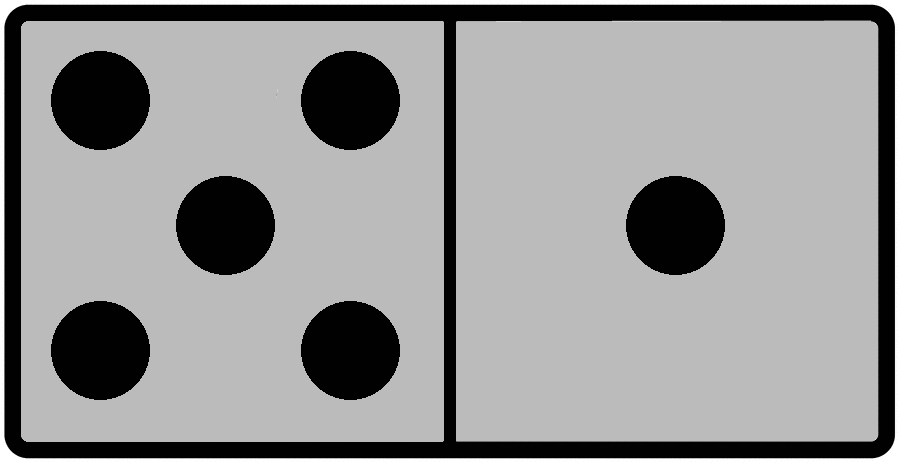
\includegraphics[width=0.3\textwidth]{gray5_1.png}
\hspace{.3in}
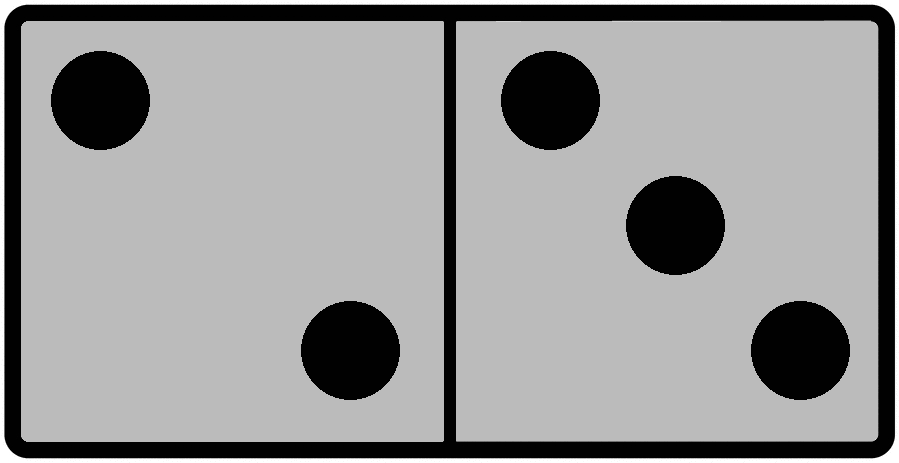
\includegraphics[width=0.3\textwidth]{gray2_3.png}
\end{center}

and your goal domino is:
\begin{center}
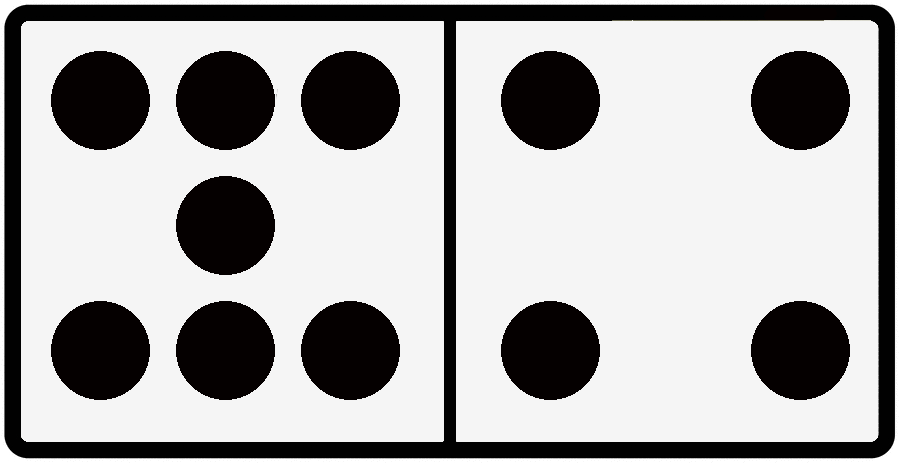
\includegraphics[width=0.3\textwidth]{white7_4.png}
\end{center}

A solution would be ``\textbf{one} and \textbf{one}.'' This means that you'll
take \textit{one} copy of the first starter domino, and \textit{one} copy of
the second, and add them together.

\begin{center}
{\LARGE Solution: \textbf{1 \& 1}}

1 \raisebox{-0.3\height}{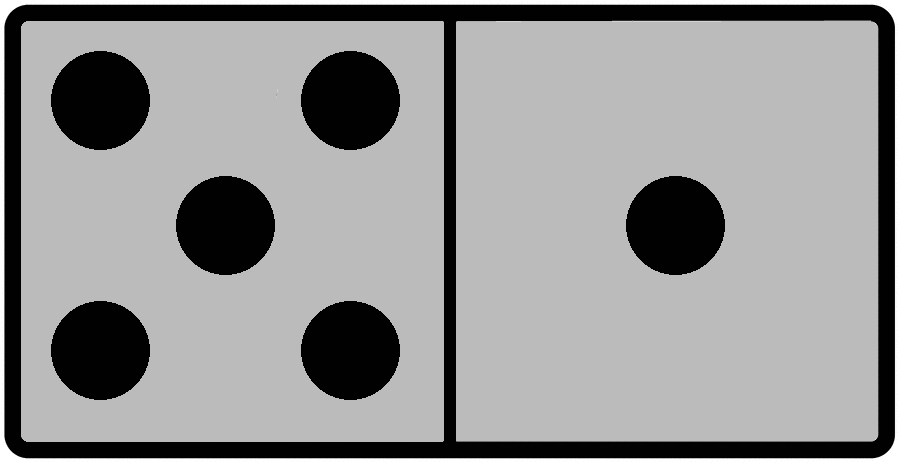
\includegraphics[width=0.1\textwidth]{gray5_1.png}} \ \& \
1 \raisebox{-0.3\height}{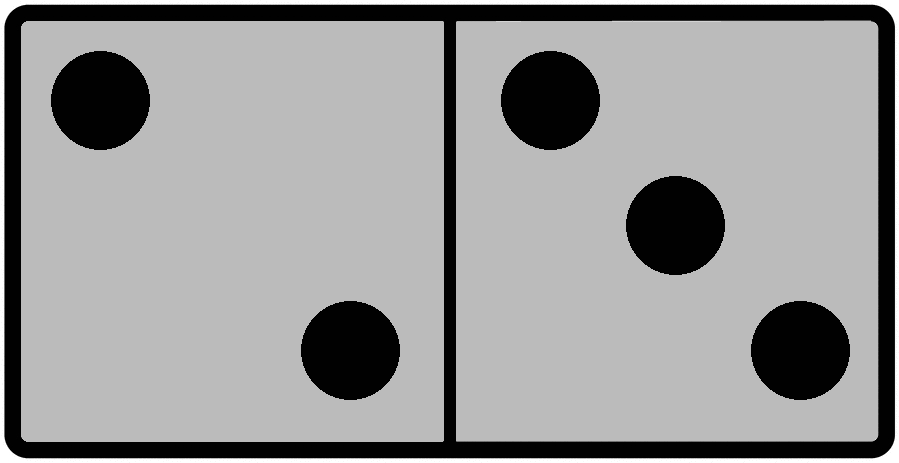
\includegraphics[width=0.1\textwidth]{gray2_3.png}} \ = \
\raisebox{-0.3\height}{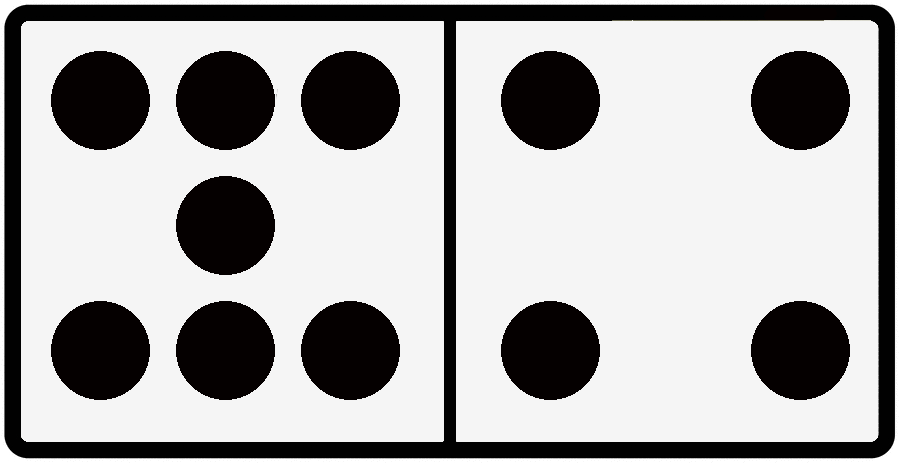
\includegraphics[width=0.1\textwidth]{white7_4.png}} \quad
\end{center}

Stare carefully at that until you master how it works; the rest of this chapter
will be a complete waste of time if this operation is not fully grasped. Adding
domino 5--1 to 2--3 means adding the left sides together, and separately adding
the right sides together, to produce a new domino 7--4 (since $5+2=7$ and
$1+3=4$).

\subsection{Actually do this}

All right, let's test your skillz. I want you to \textit{actually} work out the
answers to the following Domino Game puzzles on your own. There are six of
them, so it might take you a while (perhaps as long as 6 minutes). But it's
vital to cement your understanding of how this works...\textit{and} to set up
the crucial punchline later on in this chapter.

Answers to each puzzle are given at the end of the chapter. Maybe your answers
will not be the same as mine...or maybe they will? That itself is actually a
very important question we'll consider in a few minutes.

Enough preamble. Go!

\begin{enumerate}
\itemsep2em

\label{startDominoPuzzes}
\item Starter dominoes:
\hspace{.3in}
\raisebox{-0.3\height}{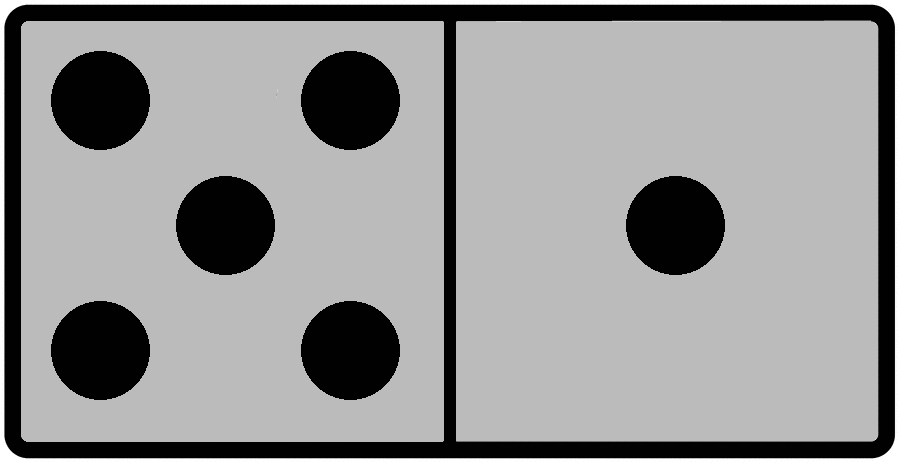
\includegraphics[width=0.2\textwidth]{gray5_1.png}}
\hspace{.1in}
\raisebox{-0.3\height}{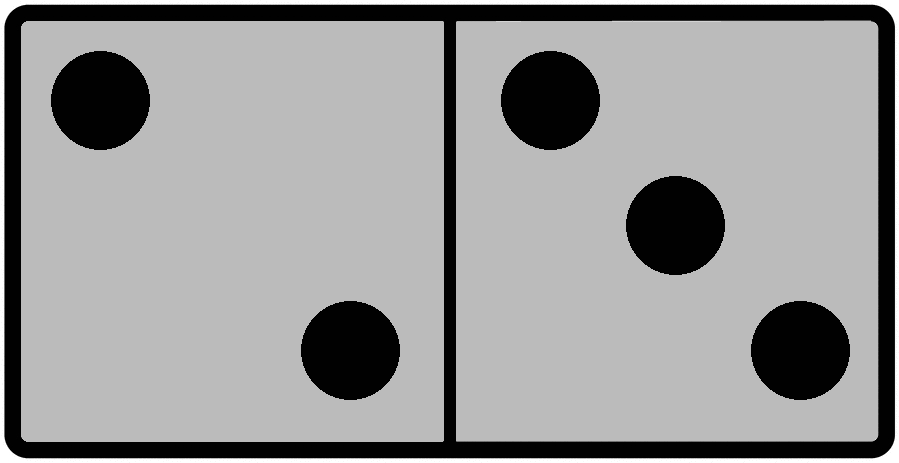
\includegraphics[width=0.2\textwidth]{gray2_3.png}}

Goal domino:
\hspace{1.1in}
\raisebox{-0.3\height}{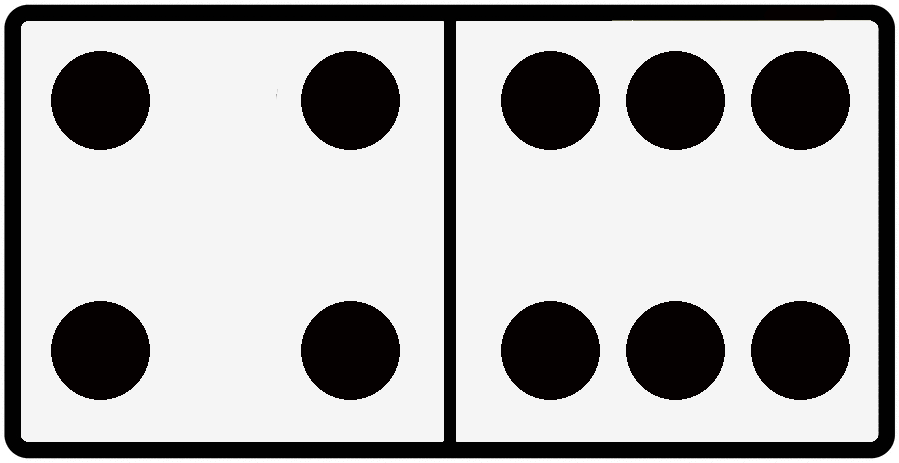
\includegraphics[width=0.2\textwidth]{white4_6.png}}

\footnotesize
(Hint: it's okay to take \textit{zero} of one of the dominoes; \textit{i.e.},
to completely ignore it.)
\normalsize

\item Starter dominoes:
\hspace{.3in}
\raisebox{-0.3\height}{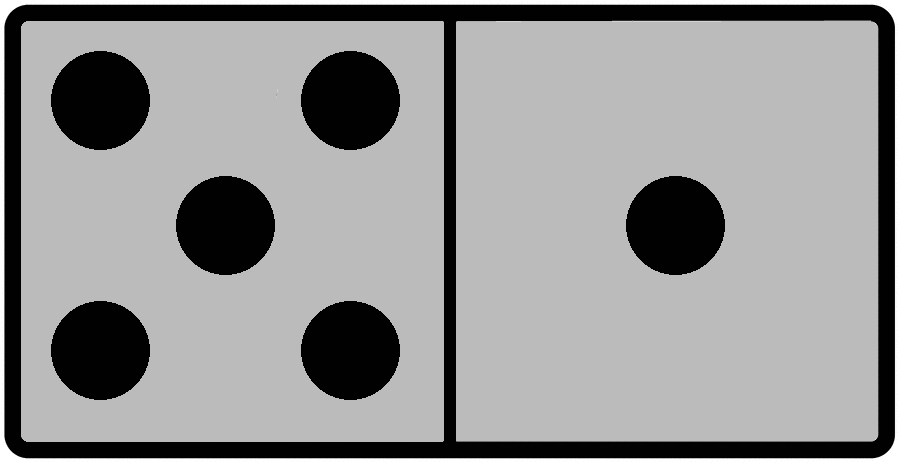
\includegraphics[width=0.2\textwidth]{gray5_1.png}}
\hspace{.1in}
\raisebox{-0.3\height}{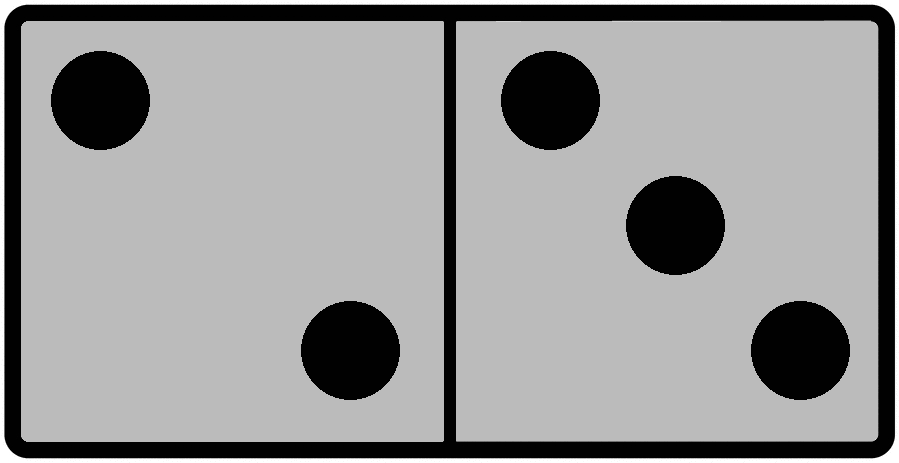
\includegraphics[width=0.2\textwidth]{gray2_3.png}}

Goal domino:
\hspace{1.1in}
\raisebox{-0.3\height}{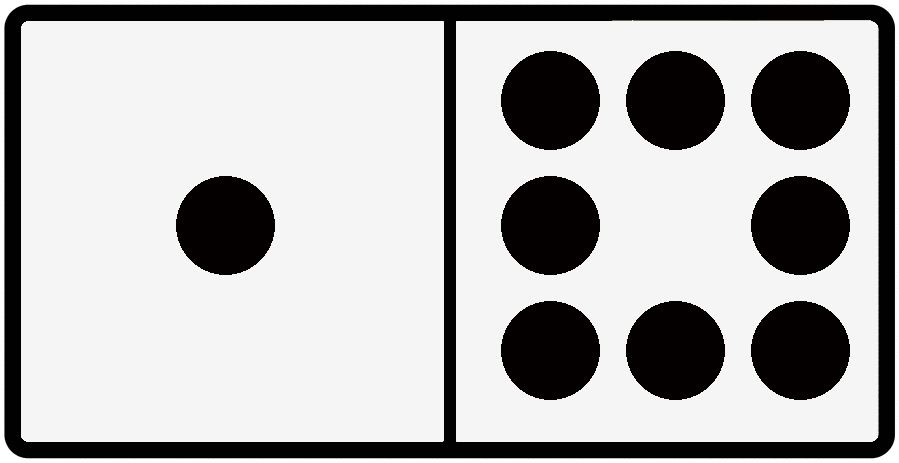
\includegraphics[width=0.2\textwidth]{white1_8.png}}

\footnotesize
(Hint: you may, if you wish, take ``a \textit{negative} number'' of one of the
dominoes. In other words, you can multiply the entire domino by a negative
number and then add it to your multiples of the other one.)
\normalsize

\item Starter dominoes:
\hspace{.3in}
\raisebox{-0.3\height}{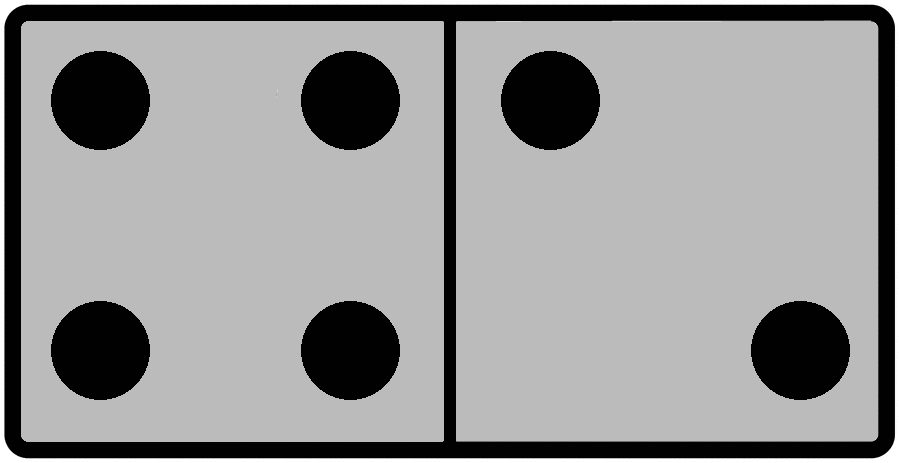
\includegraphics[width=0.2\textwidth]{gray4_2.png}}
\hspace{.1in}
\raisebox{-0.3\height}{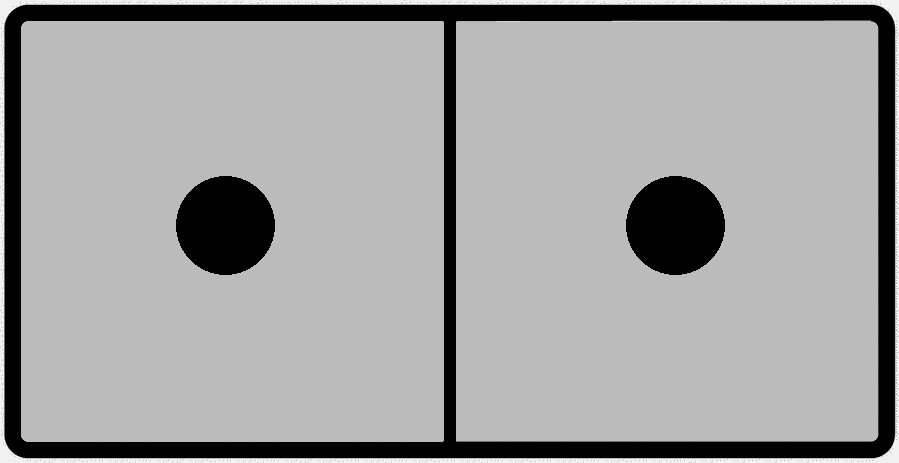
\includegraphics[width=0.2\textwidth]{gray1_1.png}}

Goal domino:
\hspace{1.1in}
\raisebox{-0.3\height}{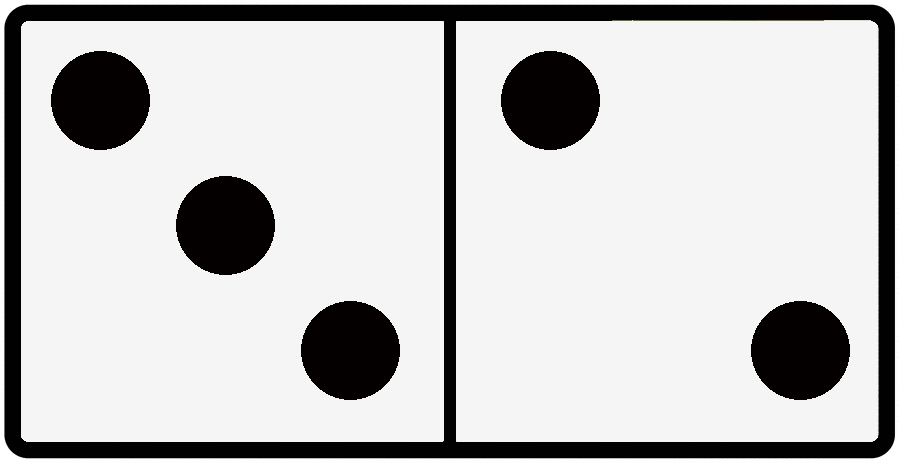
\includegraphics[width=0.2\textwidth]{white3_2.png}}

\footnotesize
(Hint: you can even take a \textit{fraction} of a domino, provided you take the
same fraction of both left and right sides. This means that just as you can
multiply an entire domino by a positive or negative number, or zero, you can
also multiply it by non-integers.)
\normalsize

\pagebreak
\item Starter dominoes:
\hspace{.3in}
\raisebox{-0.3\height}{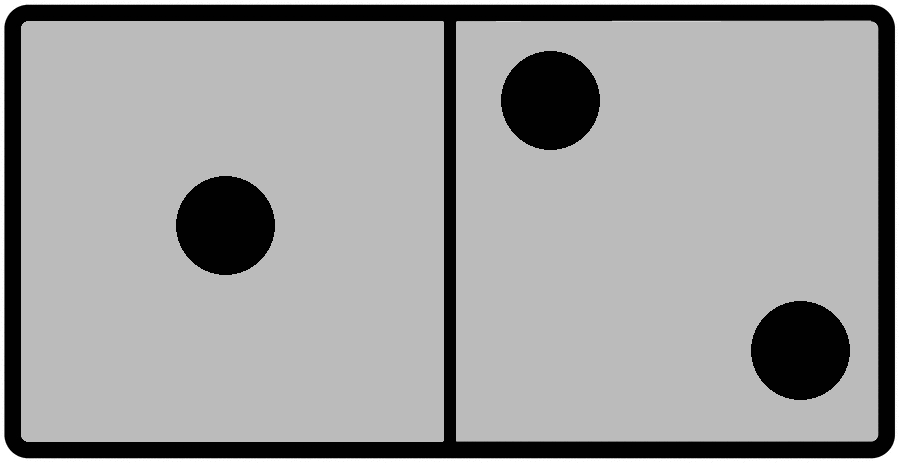
\includegraphics[width=0.2\textwidth]{gray1_2.png}}
\hspace{.1in}
\raisebox{-0.3\height}{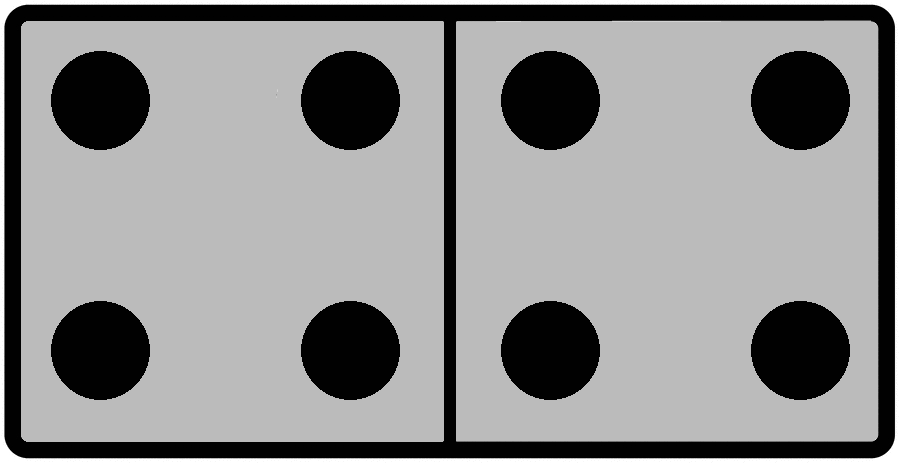
\includegraphics[width=0.2\textwidth]{gray4_4.png}}

Goal domino:
\hspace{1.1in}
\raisebox{-0.3\height}{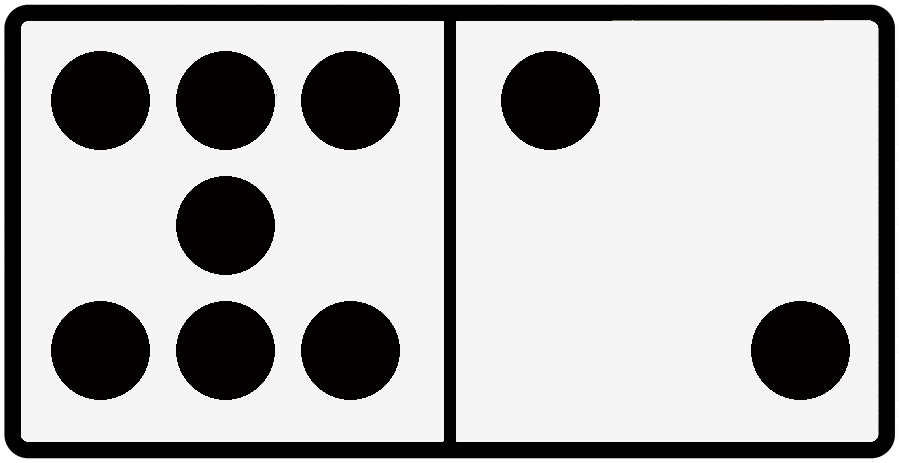
\includegraphics[width=0.2\textwidth]{white7_2.png}}

\footnotesize
(Hint: sometimes you have to go pretty far afield to get a solution, meaning a
large number of one domino and a large \textit{negative} number of the other.)
\normalsize

\item Starter dominoes:
\hspace{.3in}
\raisebox{-0.3\height}{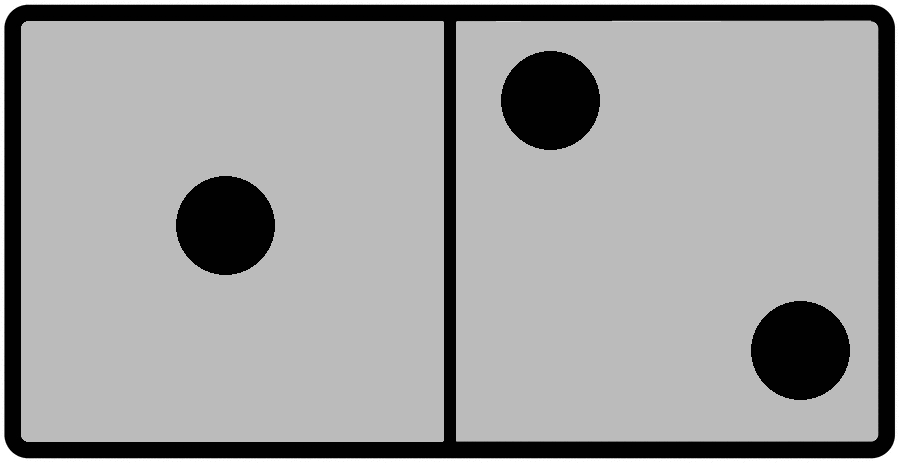
\includegraphics[width=0.2\textwidth]{gray1_2.png}}
\hspace{.1in}
\raisebox{-0.3\height}{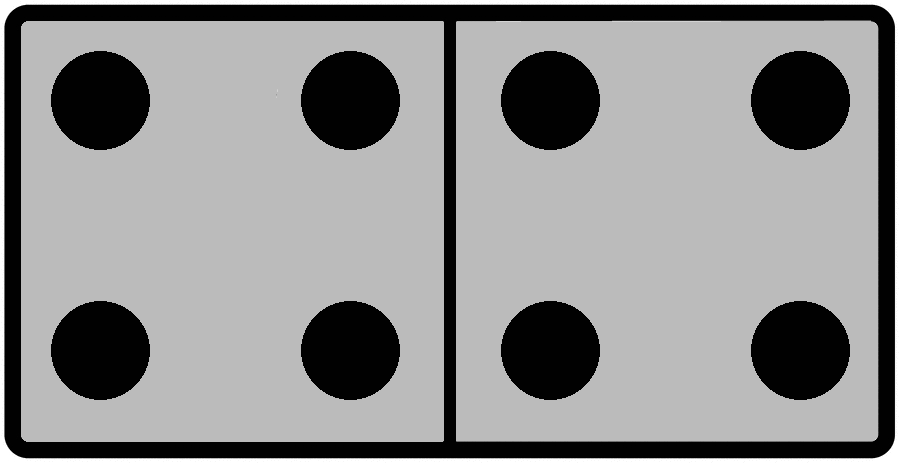
\includegraphics[width=0.2\textwidth]{gray4_4.png}}

Goal domino:
\hspace{1.1in}
\raisebox{-0.3\height}{
\includegraphics[width=0.2\textwidth]{white0_4.png}}

\footnotesize
(Hint: the goal domino can have a zero on it, just like the starter dominoes
did. But it's really no different; you just have to think creatively about how
to get the numbers to add up to zero on that side.)
\normalsize

\item Starter dominoes:
\hspace{.3in}
\raisebox{-0.3\height}{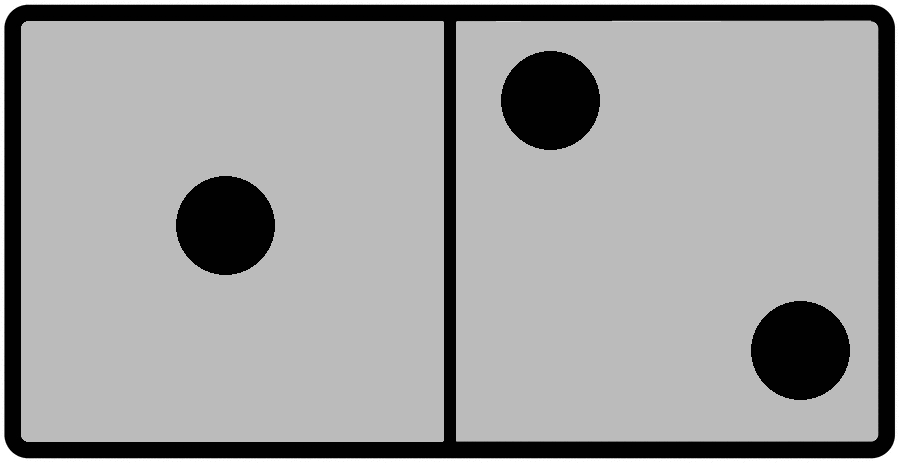
\includegraphics[width=0.2\textwidth]{gray1_2.png}}
\hspace{.1in}
\raisebox{-0.3\height}{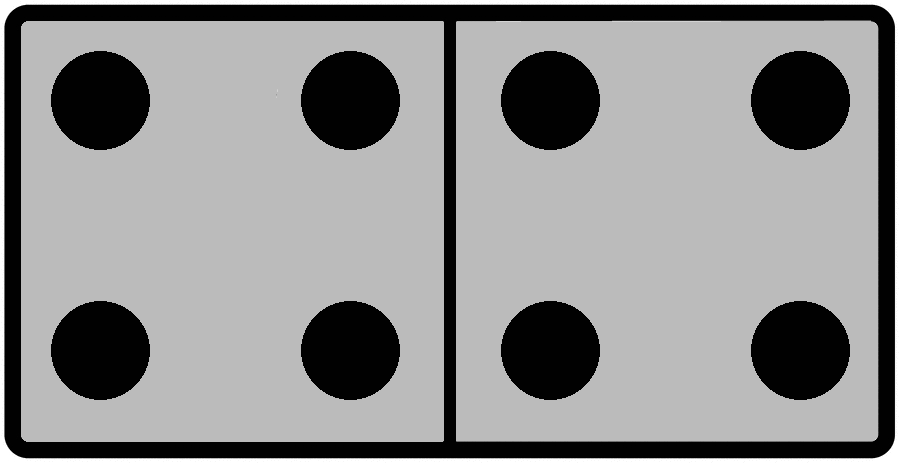
\includegraphics[width=0.2\textwidth]{gray4_4.png}}

Goal domino:
\hspace{1.1in}
\raisebox{-0.3\height}{
\includegraphics[width=0.2\textwidth]{white0_0.png}}

\footnotesize
(Hint: and yeah, the goal domino might even be \textit{completely} zero. That's
really not any different either, and in fact the solution will probably just
jump right off the page at you.)
\normalsize
\label{endDominoPuzzes}
\end{enumerate}

\subsection{Questions for curious minds}

I presume you have tried it, and hopefully succeeded at a few by trial and
error. Even if you didn't, hopefully you looked at and understood the solutions
I gave at the end of the chapter (p.~\pageref{dominoPuzzleAnswers}).

It's well worth taking a moment after all that fiddling around to consider some
interesting questions:

\begin{enumerate}
\itemsep.1em

\item Were your solutions that same as mine in each case? If so, do you think
that was just coincidence? If not, how many different solutions do you think
are possible?

\item Is it always possible to solve a puzzle like this, no matter what the
goal domino is? Or are only a small number of goal dominoes actually possible
to produce?

\item Is it always possible to solve a puzzle like this, no matter what the
starter dominoes are? Or is it only in a few cleverly crafted scenarios where
the numbers happen to work out just right?

\end{enumerate}

We'll shed light on all these matters as we move forward.

\pagebreak
\subsection*{Answers to Domino Game puzzles from
pp.~\pageref{startDominoPuzzes}-\pageref{endDominoPuzzes}}
\label{dominoPuzzleAnswers}

\begin{enumerate}
\itemsep1em

\item {Solution: \textbf{0 \& 2}}

\quad 0 \raisebox{-0.3\height}{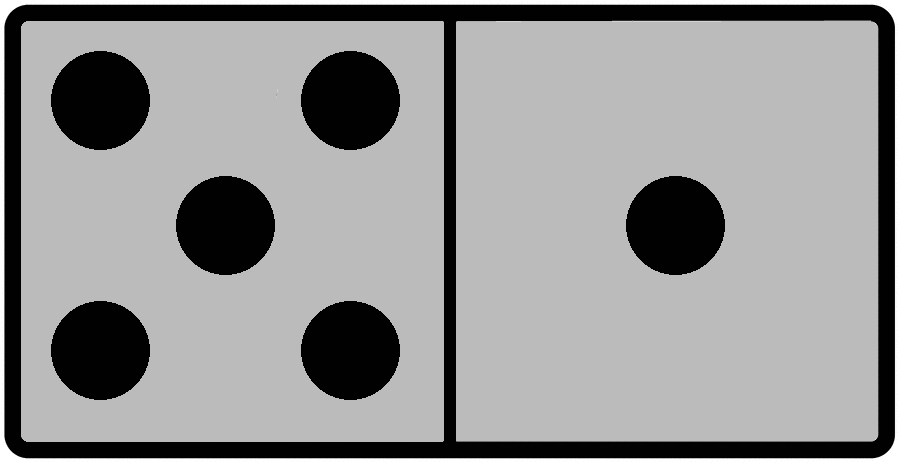
\includegraphics[width=0.1\textwidth]{gray5_1.png}} \ \& \
2 \raisebox{-0.3\height}{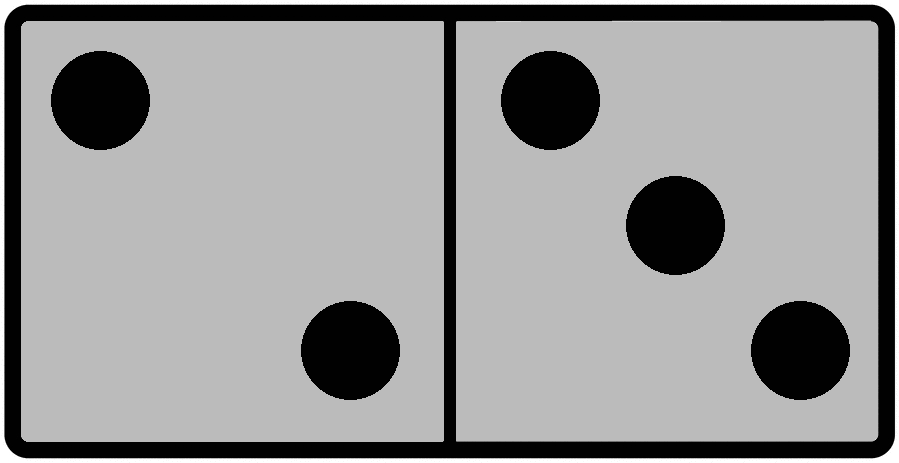
\includegraphics[width=0.1\textwidth]{gray2_3.png}} \ = \
\raisebox{-0.3\height}{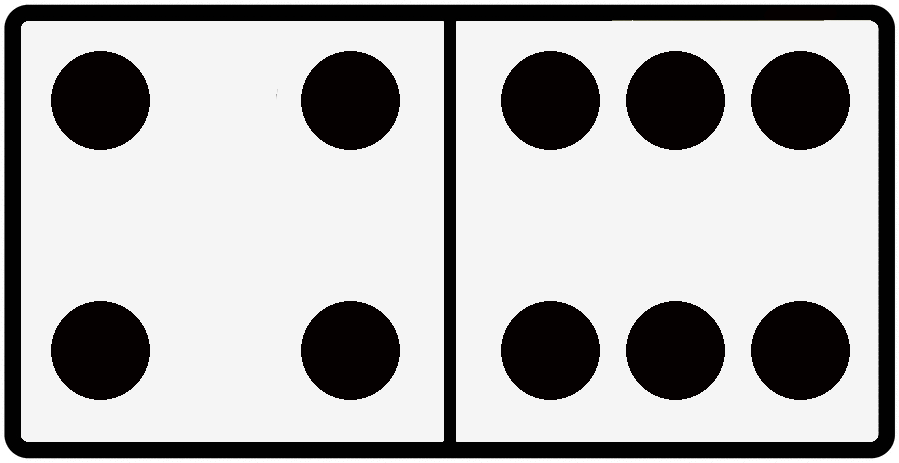
\includegraphics[width=0.1\textwidth]{white4_6.png}} \quad

\item {Solution: \textbf{--1 \& 3}}

\ $-1$ \raisebox{-0.3\height}{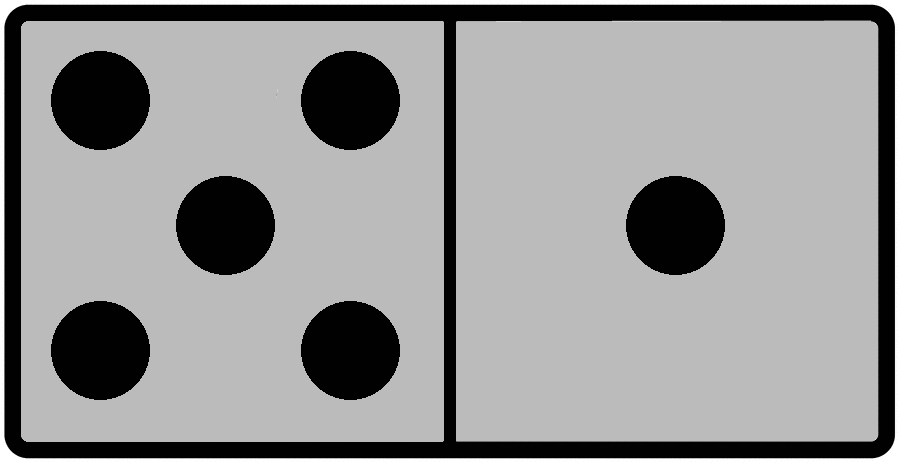
\includegraphics[width=0.1\textwidth]{gray5_1.png}} \ \& \
3 \raisebox{-0.3\height}{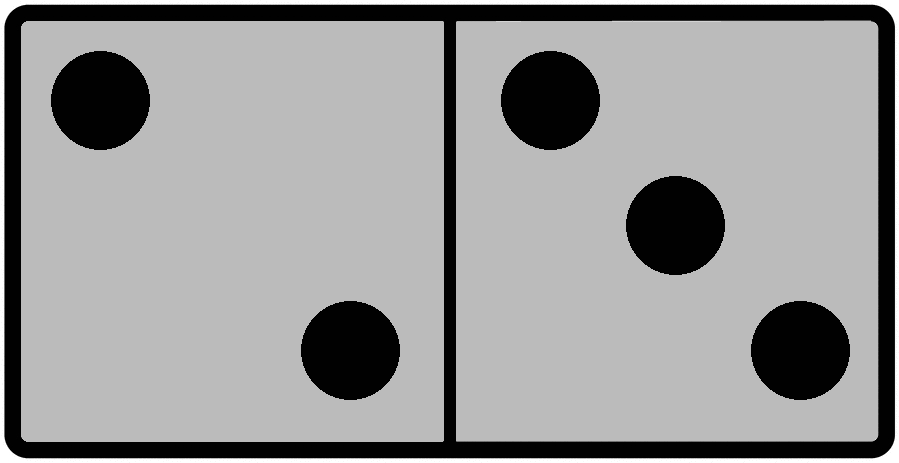
\includegraphics[width=0.1\textwidth]{gray2_3.png}} \ = \
\raisebox{-0.3\height}{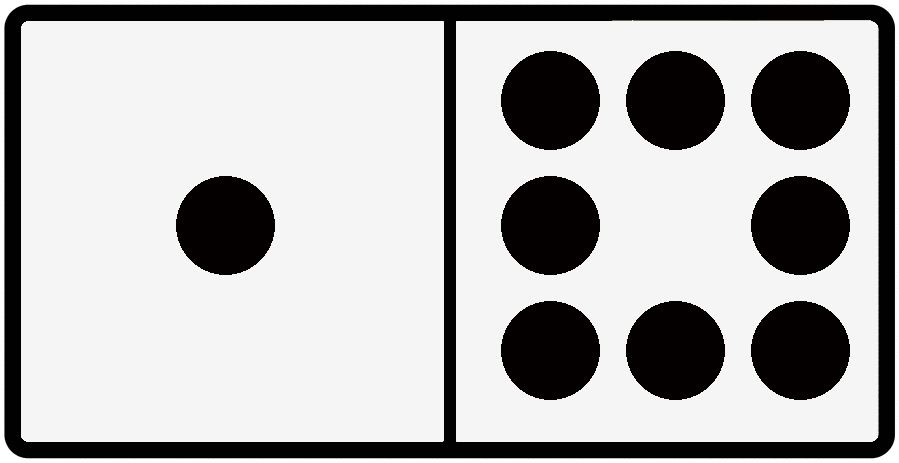
\includegraphics[width=0.1\textwidth]{white1_8.png}} \quad

\item {Solution: \textbf{$\frac{1}{2}$ \& 1}}

\quad $\frac{1}{2}$ \raisebox{-0.3\height}{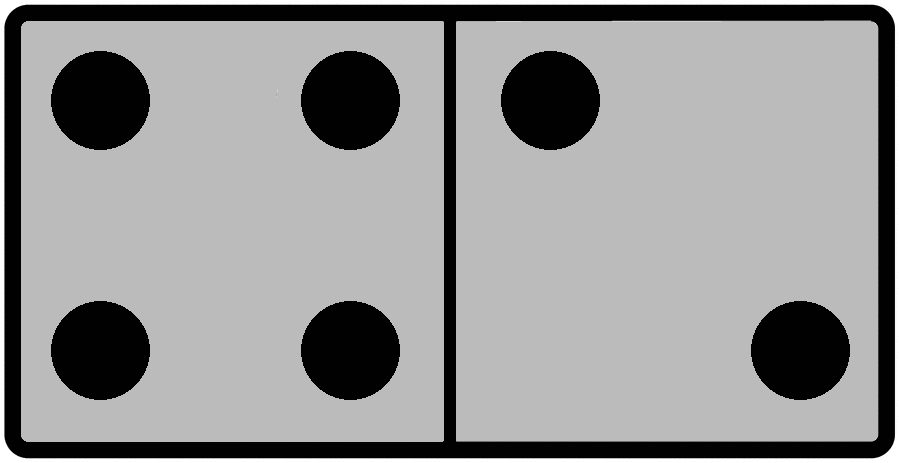
\includegraphics[width=0.1\textwidth]{gray4_2.png}} \ \& \
1 \raisebox{-0.3\height}{\includegraphics[width=0.1\textwidth]{gray1_1.png}} \ = \
\raisebox{-0.3\height}{\includegraphics[width=0.1\textwidth]{white3_2.png}} \quad

\item {Solution: \textbf{-5 \& 3}}

\ $-5$ \raisebox{-0.3\height}{\includegraphics[width=0.1\textwidth]{gray1_2.png}} \ \& \
3 \raisebox{-0.3\height}{\includegraphics[width=0.1\textwidth]{gray4_4.png}} \ = \
\raisebox{-0.3\height}{\includegraphics[width=0.1\textwidth]{white7_2.png}} \quad

\item {Solution: \textbf{4 \& --1}}

\quad 4 \raisebox{-0.3\height}{\includegraphics[width=0.1\textwidth]{gray1_2.png}} \&
$-1$ \raisebox{-0.3\height}{\includegraphics[width=0.1\textwidth]{gray4_4.png}} \ = \
\raisebox{-0.3\height}{\includegraphics[width=0.1\textwidth]{white0_4.png}} \quad

\item {Solution: \textbf{0 \& 0}}

\quad 0 \raisebox{-0.3\height}{\includegraphics[width=0.1\textwidth]{gray1_2.png}} \ \& \
0 \ \raisebox{-0.3\height}{\includegraphics[width=0.1\textwidth]{gray4_4.png}} \ = \
\raisebox{-0.3\height}{\includegraphics[width=0.1\textwidth]{white0_0.png}} \quad

\end{enumerate}


\chapter{Matrices}

It's now time for the granddaddy of all linear algebra entities: the
\textbf{matrix}. When we've finished this part of our climb, you'll actually be
able to see the summit we'll eventually reach.

By the way, the plural of \textit{matrix} is \textbf{matrices} (pronounced
MAY-trih-sees), kind of like the plural of \textit{index} is \textit{indices.}
But don't forget the singular is still ``\textit{matrix}!'' Don't let me (or
anyone else) catch you uttering the non-word ``matrice'' -- you'll sound like a
dweeb and drive me up a wall.

\section{Row and column vectors}
\index{vector}

Up to now, a vector has simply been a vector. I haven't made a big deal about
how you write it on the page. We've been free to write a vector
$\overrightarrow{\textbf{x}}$ with the three elements 6, 2, and 9 in either of
these ways:

\vspace{-.15in}
\begin{center}
\begin{tabular}{ccc}
$\overrightarrow{\textbf{x}}$ = \textbf{[}$\ 6\ \ 2\ \ 9\ $\textbf{]} &
\quad\quad \textit{...or...} \quad\quad &
$\overrightarrow{\textbf{x}}$ = $\begin{bmatrix} 6 \\ 2 \\ 9 \end{bmatrix}$ \ 
\end{tabular}
\end{center}
\vspace{-.15in}

\index{function}

Or heck, you could even write it diagonally if you want. This flexibility is
because all that really matters is the \textit{function} view of a vector that
we discussed in section~\ref{vectorIsFunction}. All that ultimately matters is
that you associate the correct index number with the correct element. However I
might draw $\overrightarrow{\textbf{x}}$ on paper, if I asked you for the value
of ``element \#0,'' you'd say 6, and if I asked for ``element \#2,'' you'd say
9. The way it looks has been immaterial up until now.

\index{row vector}
\index{column vector}

That will still be true sometimes. But beginning with this chapter, it's going
to sometimes turn out to matter whether or not we think of a vector as a
\textbf{row vector} (the left-hand-side version of
$\overrightarrow{\textbf{x}}$, above) or a \textbf{column vector} (the
right-hand-side). Memorize these terms: they matter, and you'll have to have
them on the tip of your neural cortex. A row goes horizontally, side-to-side;
and a column goes vertically, up-to-down.

I'll try to always be very careful to emphasize the row vs.~column nature of a
vector in those cases where it turns out to matter.

\index{default}

By the way, one surprising thing (at least, it was to me) is that the
``default'' is for an unspecified vector to be treated as a \textit{column}
vector, not a row. Column vectors take up more room on the page, and aren't as
natural when you're writing on paper, which I guess is why it surprised me. At
any rate, whenever a vector is under discussion, try to visualize it as an
up-and-down column of entries, unless the accompanying text explicitly says
otherwise.

\section{The matrix}

\index{matrix (plural: matrices)}

At last, the matrix. This will seem underwhelming at first, but \textit{boy}
does it pack a wallop.

A matrix is simply a two-dimensional rectangular grid of entries, kind of like
a spreadsheet. We'll use capital letters to designate them, with no special
arrow-like or other adornment. Here's our first example:

\vspace{-.15in}
\begin{align*}
A =
\begin{bmatrix}
5 &-7 &3 &9 \\
18 &4 &1 &1 \\
3 &-3 &\pi &4 \\
\end{bmatrix}
\end{align*}
\vspace{-.15in}

\index{dimension}

Matrices are always rectangular, but not always square. The $A$ matrix is
called a ``$3\times 4$'' (three-by-four) matrix, since it has three
\textbf{row}s and four \textbf{column}s. We say that $3\times 4$ are the
matrix's \textbf{dimensions}. Again, it's important to master all this
terminology. When giving the dimensions of a matrix, you always list the number
of rows first, and then the number of columns.

\index{index number}

To specify an individual element, we need \textit{two} indices instead of just
one as we did for a vector. We'll use Python-style numbering (starting with 0)
and write the row and column as a two-part comma-separated subscript:

\vspace{-.15in}
\begin{align*}
A_{0,0} &= 5 \\
A_{1,0} &= 18 \\
A_{0,3} &= 9 \\
A_{2,2} &= \pi \\
\end{align*}
\vspace{-.25in}

Just practice first moving down to the correct row, then moving over to the
correct column, and you'll be fine.

\subsection{Labels}

\index{label}

As with vectors, we won't always use index numbers to designate rows and
columns: sometimes we'll use labels. Check out this matrix $W$ (for
``weather''):

\vspace{-.4in} 
\begin{adjustwidth}{}{60pt}
\begin{center}
\begin{multicols}{2}
\begin{flushright}
\hspace*{1cm} \\
\hspace*{1cm} \\
\footnotesize{D.C.} \\
\footnotesize{Fredericksburg} \\
\footnotesize{Richmond} \\
\end{flushright}
\columnbreak
\vspace{-1.5in} 
\begin{align*}
\begin{bmatrix}
81 \ & \ 86 \ & \ 78 \ & \ 74 \ & \ 77 \\
83 \ & \ 86 \ & \ 79 \ & \ 79 \ & \ 82 \\
82 \ & \ 86 \ & \ 84 \ & \ 87 \ & \ 87 \\
\end{bmatrix}
\end{align*}
\vspace{-.15in}
\scriptsize{Mon} \ \  \scriptsize{Tue} \ \ \scriptsize{Wed} \ \ \scriptsize{Thu} \ \ \scriptsize{Fri} \\
\end{multicols}
\end{center}
\end{adjustwidth}
\vspace{-.15in}

Here we're using city names for the row labels, and days of the week as the
column labels. It's still easy peasy to interpret -- how hot did it get in the
nation's capital on Tuesday? 86\textdegree, of course. Using the same subscript
notation as above, we could say:

\vspace{-.15in}
\begin{align*}
W_{\textrm{D.C.},\textrm{Mon}} &= 81 \\
W_{\textrm{Fredericksburg},\textrm{Wed}} &= 79 \\
W_{\textrm{Fredericksburg},\textrm{Thu}} &= 79 \\
W_{\textrm{Richmond},\textrm{Thu}} &= 87 \\
&\vdots \\
\end{align*}

and so forth. D.C. and Fred had a bit of a cool-down midweek, thank God, while
Richmond was all the while cooking in the upper 80's.

\section{A matrix is also a function}

\index{function}
Remember back in section~\ref{vectorIsFunction} (p.~\pageref{vectorIsFunction})
when I explained that a vector, viewed in a sufficiently weird way, was
actually a function? The same thing is true for matrices, just by adding one
more input to the function.

Put another way, let's consider the row labels (or numbers, if we want to be
boring) as the set $C$ (for ``cities''). And let's consider the column labels
as the set $D$ (for ``days-of-the-week''). Then, you can see that a matrix is
precisely maps a pair of a city and a day to a high temperature. (The high
temperatures are in the set $\mathbb{R}$, which are the real numbers.) In
symbols, $W$ is defined as this function:

\vspace{-.15in}
\begin{align*}
W : C \times D \rightarrow \mathbb{R}
\end{align*}
\vspace{-.15in}

\index{domain}
\index{codomain}
\index{Cartesian product}
Recall that function syntax. $W$ is the name of the function. The part before
the arrow is the \textbf{domain} of the function: the set which its inputs are
drawn from. Since it's the Cartesian product of two sets (cities and days) this
domain is really all the ordered pairs of cities-and-days, like (D.C., Thurs)
and (Richmond, Monday). The function takes any ordered pair like that and gives
you a number telling you how hot that city was on that day. It's a snap when
seen this way.


\section{Matrix operations}

Just as section~\ref{vectorOps} listed the permissible actions we could perform
on vectors (and scalars), so this section lists the operations we can perform
on matrices (and vectors, and scalars). There's one other big one which I'll
save for entire separate chapter, but there are still four useful ones we'll
cover here.

\subsection{Operation \#1: scalar-matrix multiplication}

This one's a piece of cake. Recall that multiplying a scalar by a vector
amounted to multiplying the scalar by each of its elements, producing a vector
of the same dimension. Same here: we get a matrix of the same dimension by
multiplying individually:

\vspace{-.15in}
\begin{align*}
4 \cdot
\begin{bmatrix}
3 & 2 & 9 \\
1 & -1 & 0 \\
\end{bmatrix}
=
\begin{bmatrix}
12 & 8 & 36 \\
4 & -4 & 0 \\
\end{bmatrix}.
\end{align*}
\vspace{-.15in}

Sometimes we'll put a dot between the two, as above, though we'll often omit
that and just write the scalar and matrix side-by-side. Either way, it means
scalar-matrix multiplication.

\subsection{Operation \#2: matrix addition}

Also a piece of cake, and just what you'd expect:

\vspace{-.15in}
\begin{align*}
\begin{bmatrix}
4 & 1 \\
1 & -2 \\
3 & 18 \\
\end{bmatrix}
\begin{bmatrix}
1 & 2 \\
5 & 2 \\
-10 & -10 \\
\end{bmatrix}
+
\begin{bmatrix}
5 & 3 \\
6 & 0 \\
-7 & 8 \\
\end{bmatrix}.
\end{align*}
\vspace{-.15in}

The only hard part is not going cross-eyed as you zigzag your eyeballs across
the page to match up entries.

As with vector addition, you simply can't add two matrices at all if they don't
have the same dimensions. Also just like vectors, we can \textit{subtract} one
matrix from another just by adding the first matrix to ``$-1$ times the second
matrix.''

%transpose
%2x3 transpose gives us 3x2.  (Ai,j = ATj,i)
%
%use transpose on a row vector to get a column vector.
%(Treating the vector as a one-row / one-col matrix when we do this)
%
%
%matrix-vector multiplication. not what you'd expect. not even the kind of
%result you'd expect.
%
%Make A a 4x2, x a column vector 2x1.
%if mxn matrix, you need a n-dimensional column vector (or "nx1 matrix")
%weird! # of rows of one must be # of columns of the other.
%get an mx1 answer!
%
%two different ways to think about this A dot xvector.
%
%1. All the dot products of the vector with the matrix's rows.
%2. A linear combination of the matrix's columns (with the vector's elements as
%coefficients.)
%
%Show the second thing all worked out as the linear combo of columns.
%
%
%Why think about it as way 1? Jezebel col vector, matrix of all the guys (heck,
%let's put guys surveys in columns too, then that requires transpose
%
%
%Why think about it in way 2? Recipes matrix. each column is one recipe, each
%row is an ingredient. Vector shows how many of each recipe you want to make.
%


\backmatter
\printindex

\end{document}
